\documentclass[11pt]{report}
\usepackage[utf8]{inputenc}	% Para caracteres en español
\usepackage{amsmath,amsthm,amsfonts,amssymb,amscd}
\usepackage{multirow,booktabs}
\usepackage[table]{xcolor}
\usepackage{fullpage}
\usepackage{lastpage}
\usepackage{enumitem}
\usepackage{fancyhdr}
\usepackage{mathrsfs}
\usepackage{wrapfig}
\usepackage{setspace}
\usepackage{hyperref}
\usepackage{calc}
\usepackage{multicol}
\usepackage{cancel}
\usepackage[retainorgcmds]{IEEEtrantools}
\usepackage[margin=3cm]{geometry}
\usepackage{amsmath}
\newlength{\tabcont}
\setlength{\parindent}{0.0in}
\setlength{\parskip}{0.05in}
\usepackage{empheq}
\usepackage{framed}
\usepackage[most]{tcolorbox}
\usepackage{xcolor}
\colorlet{shadecolor}{orange!15}
\parindent 0in
\parskip 12pt
\geometry{margin=1in, headsep=0.25in}
\theoremstyle{definition}
\usepackage{pdfpages}
\newtheorem{defn}{Definition}
\newtheorem{reg}{Rule}
\newtheorem{exer}{Exercise}
\newtheorem{note}{Note}
\usepackage{fancyhdr}\usepackage{xcolor}\usepackage{amsmath}\usepackage{amssymb}\pagestyle{fancy}\rhead{}
\newtheorem{theorem}{Theorem}[subsection]
\theoremstyle{definition}
\newtheorem{definition}[theorem]{Definiton}
\newtheorem{example}[theorem]{Example}
\newtheorem{corollary}[theorem]{Corollary}
\newtheorem{lemma}[theorem]{Lemma}
\title{Chapter 9 Review Notes}
\begin{document}
\thispagestyle{empty}
{\LARGE \bf AER 210 Lecture Notes}\\
{\large Hei Shing Cheung}\\
Vector Calculus \& Fluid Mechanics, Fall 2025 \hfill AER210\\
\\
The up-to-date version of this document can be found at \url{https://github.com/HaysonC/skulenotes}\\

\chapter{Vector Calculus}

% set section counter from 15 
\setcounter{section}{13}
\paragraph{Note} the section numbering is based on Stewart's book.

\section{Partial Derivatives}
\paragraph{Continuing from Calc II} We consider Taylor series of multivariable functions, and we would need to consider partial derivatives.

\subsection{Taylor Series for Multivariable Functions}

\begin{keybox}
	\textbf{Key Equations:}
\begin{itemize}
    \item Multivariable Taylor (about $(x_0,y_0)$): $\displaystyle f(x,y) = f_0 + \sum_i f_i\Delta x_i + \tfrac12\sum_{i,j} f_{ij}\Delta x_i\Delta x_j + \cdots$
    \item 2D form: $\displaystyle f(x_0{+}\Delta x,y_0{+}\Delta y) = f_0 + f_x\Delta x + f_y\Delta y + \tfrac12(f_{xx}\Delta x^2 + 2f_{xy}\Delta x\Delta y + f_{yy}\Delta y^2)+\cdots$
\end{itemize}
	\textbf{Tips:}
\begin{itemize}
    \item Use a line path $(x,y)=(x_0,y_0)+t(\Delta x,\Delta y)$ to reduce to 1D.
    \item Hessian controls the quadratic term and local shape (min/max/saddle with tests later).
\end{itemize}
\end{keybox}

\begin{shaded}
    \subsubsection{Review. Taylor Series for Single Variable Functions}
    Let $f(x)$ be a function that is infinitely differentiable at $x = a$. The Taylor series of $f(x)$ about the point $x = a$ is given by:
    \begin{equation}
        f(x) = f(a) + f'(a)(x-a) + \frac{f''(a)}{2!}(x-a)^2 + \frac{f'''(a)}{3!}(x-a)^3 + \cdots = \sum_{n=0}^{\infty} \frac{f^{(n)}(a)}{n!} (x-a)^n
    \end{equation}

    Also, consider the taylor approximation of $f(x + \Delta x)$ about $x$: 
    \begin{equation}
        f(x + \Delta x) = f(x) + f'(x)\Delta x + \frac{f''(x)}{2!}(\Delta x)^2 + \frac{f'''(x)}{3!}(\Delta x)^3 + \cdots = \sum_{n=0}^{\infty} \frac{f^{(n)}(x)}{n!} (\Delta x)^n
    \end{equation}
\end{shaded}
\begin{definition}[Taylor Series for Multivariable Functions]
    Let $f(x,y)$ be a function that is infinitely differentiable at the point $(a,b)$. Consider the increment $\Delta x$ in the $x$-direction and $\Delta y$ in the $y$-direction centred at $(x_0,y_0)$. We have the following parametric equations:
    $$
        \begin{cases}
            x = x_0 + \Delta x t \\
            y = y_0 + \Delta y t
        \end{cases} \quad t \in [0,1]
    $$
    Define a new function $g(t) = f(x_0 + \Delta x t, y_0 + \Delta y t)$, which is a single-variable function in terms of $t$. We can then apply the Taylor series for single-variable functions to $g(t)$ about $t = 0$:
    $$
        g(t) = g(0) + g'(0)t + \frac{g''(0)}{2!}t^2 + \frac{g'''(0)}{3!}t^3 + \cdots = \sum_{n=0}^{\infty} \frac{g^{(n)}(0)}{n!} t^n
    $$
    Using the chain rule, we can compute the taylor series of $f(x,y)$ about the point $(x_0,y_0)$:
    \begin{align}
        f(x_0 + \Delta x, y_0 + \Delta y) &= f(x_0,y_0) + \left( \frac{\partial f}{\partial x} \Delta x + \frac{\partial f}{\partial y} \Delta y \right) \nonumber \\
        & + \frac{1}{2!} \left( \frac{\partial^2 f}{\partial x^2} (\Delta x)^2 + 2\frac{\partial^2 f}{\partial x \partial y} \Delta x \Delta y + \frac{\partial^2 f}{\partial y^2} (\Delta y)^2 \right) + \cdots \\
        &= f(x_0,y_0) + \sum_{n=1}^{\infty} \sum_{k=0}^n \frac{1}{k!(n-k)!} \frac{\partial^n f}{\partial x^k \partial y^{n-k}} (\Delta x)^k (\Delta y)^{n-k}
    \end{align}
    Or equivalently, we can write:
    \begin{equation}
        f(x,y) = f(x_0,y_0) + \sum_{n=1}^{\infty} \sum_{k=0}^n \frac{1}{k!(n-k)!} \frac{\partial^n f}{\partial x^k \partial y^{n-k}} (x - x_0)^k (y - y_0)^{n-k}
    \end{equation}
    We could also use the fact:
    $$
        \frac{1}{k!(n-k)!} = \frac{1}{n!} \binom{n}{k}
    $$
    we rewrite the above equations, such that we can use the pascal's triangle to help us remember the coefficients:
    \begin{equation}
        f(x,y) = f(x_0,y_0) + \sum_{n=1}^{\infty} \frac{1}{n!} \sum_{k=0}^n \binom{n}{k} \frac{\partial^n f}{\partial x^k \partial y^{n-k}} (x - x_0)^k (y - y_0)^{n-k}
    \end{equation}

    WLOG, this can be extended to functions of more than two variables.
\end{definition}

\begin{example}[Thrid (3$^{\text{rd}}$) order Taylor Polynomial]
    For some function $f(x,y)$, the third order Taylor polynomial about the point $(x_0,y_0)$ is given by:
    \begin{align*}
        f(x,y) &= f(x_0,y_0) + \left( \frac{\partial f}{\partial x} (x - x_0) + \frac{\partial f}{\partial y} (y - y_0) \right) \\
        &\quad + \frac{1}{2!} \left( \frac{\partial^2 f}{\partial x^2} (x - x_0)^2 + 2\frac{\partial^2 f}{\partial x \partial y} (x - x_0)(y - y_0) + \frac{\partial^2 f}{\partial y^2} (y - y_0)^2 \right) \\
        &\quad + \frac{1}{3!} \left( \frac{\partial^3 f}{\partial x^3} (x - x_0)^3 + 3\frac{\partial^3 f}{\partial x^2 \partial y} (x - x_0)^2 (y - y_0) + 3\frac{\partial^3 f}{\partial x \partial y^2} (x - x_0)(y - y_0)^2 + \frac{\partial^3 f}{\partial y^3} (y - y_0)^3 \right) \\
        &\quad + O\left( ||(x - x_0, y - y_0)||^4 \right)
    \end{align*}
    where $O\left( ||(x - x_0, y - y_0)||^4 \right)$ represents the higher order terms that are of order 4 or higher in the Taylor series expansion.
\end{example}

\begin{example}[Three Variable Case]
    For some function $f(x,y,z)$, the second order Taylor polynomial about the point $(x_0,y_0,z_0)$ is given by:
    \begin{align*}
        f(x,y,z) &= f(x_0,y_0,z_0) + \left( \frac{\partial f}{\partial x} (x - x_0) + \frac{\partial f}{\partial y} (y - y_0) + \frac{\partial f}{\partial z} (z - z_0) \right) + \\
        &\quad \frac{1}{2!} \left( \frac{\partial^2 f}{\partial x^2} (x - x_0)^2 + 2\frac{\partial^2 f}{\partial x \partial y} (x - x_0)(y - y_0) + 2\frac{\partial^2 f}{\partial x \partial z} (x - x_0)(z - z_0) + \right. \\
        &\quad \left. \frac{\partial^2 f}{\partial y^2} (y - y_0)^2 + 2\frac{\partial^2 f}{\partial y \partial z} (y - y_0)(z - z_0) + \frac{\partial^2 f}{\partial z^2} (z - z_0)^2 \right) + \\
        &\quad O\left( ||(x - x_0, y - y_0, z - z_0)||^3 \right)
    \end{align*}
    where $O\left( ||(x - x_0, y - y_0, z - z_0)||^3 \right)$ represents the higher order terms that are of order 3 or higher in the Taylor series expansion.
    
\end{example}

\begin{example}
    \textit{Find the second order Taylor polynomial of $f(x,y) = \sqrt{x^2 + y^3}$ about the point $(1,2)$.}
    
    First, we compute the necessary partial derivatives at the point $(1,2)$:
    \begin{align*}
        f(x,y) &= \sqrt{x^2 + y^3} \implies f(1,2) = \sqrt{1^2 + 2^3} = \sqrt{9} = 3 \\
        f_x(x,y) &= \frac{x}{\sqrt{x^2 + y^3}} \implies f_x(1,2) = \frac{1}{3} \\
        f_y(x,y) &= \frac{3y^2}{2\sqrt{x^2 + y^3}} \implies f_y(1,2) = \frac{6}{3} = 2 \\
        f_{xx}(x,y) &= \frac{y^3}{(x^2 + y^3)^{3/2}} \implies f_{xx}(1,2) = \frac{8}{27} \\
        f_{yy}(x,y) &= \frac{3x^2}{4(x^2 + y^3)^{3/2}} \implies f_{yy}(1,2) = \frac{3}{27} = \frac{1}{9} \\
        f_{xy}(x,y) &= -\frac{3xy^2}{2(x^2 + y^3)^{3/2}} \implies f_{xy}(1,2) = -\frac{6}{27} = -\frac{2}{9}
    \end{align*}
    Now, we can plug these values into the second order Taylor polynomial formula:
    \begin{align*}
        f(x,y) &\approx f(1,2) + f_x(1,2)(x-1) + f_y(1,2)(y-2) \\
        &\quad + \frac{1}{2} \left( f_{xx}(1,2)(x-1)^2 + 2f_{xy}(1,2)(x-1)(y-2) + f_{yy}(1,2)(y-2)^2 \right) \\
        &\approx 3 + \frac{1}{3}(x-1) + 2(y-2) + \frac{1}{2} \left( \frac{8}{27}(x-1)^2 - \frac{4}{9}(x-1)(y-2) + \frac{1}{9}(y-2)^2 \right)
    \end{align*}
\end{example}

\begin{example}
    \textit{Find the third-order taylor expansion for $f(x,y) = e^{x-2y}$ about the point $(0,0)$.}
    
    \textbf{Method 1 (using multivariable taylor series)} We compute the necessary partial derivatives at the point $(0,0)$:
    \begin{align*}
        f(x,y) &= e^{x-2y} \implies f(0,0) = e^0 = 1 \\
        f_x(x,y) &= e^{x-2y} \implies f_x(0,0) = 1 \\
        f_y(x,y) &= -2e^{x-2y} \implies f_y(0,0) = -2 \\
        f_{xx}(x,y) &= e^{x-2y} \implies f_{xx}(0,0) = 1 \\
        f_{yy}(x,y) &= 4e^{x-2y} \implies f_{yy}(0,0) = 4 \\
        f_{xy}(x,y) &= -2e^{x-2y} \implies f_{xy}(0,0) = -2 \\
        f_{xxx}(x,y) &= e^{x-2y} \implies f_{xxx}(0,0) = 1 \\
        f_{yyy}(x,y) &= -8e^{x-2y} \implies f_{yyy}(0,0) = -8 \\
        f_{xxy}(x,y) &= -2e^{x-2y} \implies f_{xxy}(0,0) = -2 \\
        f_{xyy}(x,y) &= 4e^{x-2y} \implies f_{xyy}(0,0) = 4
    \end{align*}
    Now, we can plug these values into the third order Taylor polynomial formula:
    \begin{align*}
        f(x,y) &\approx f(0,0) + f_x(0,0)x + f_y(0,0)y \\
        &\quad + \frac{1}{2} \left( f_{xx}(0,0)x^2 + 2f_{xy}(0,0)xy + f_{yy}(0,0)y^2 \right) \\
        &\quad + \frac{1}{6} \left( f_{xxx}(0,0)x^3 + 3f_{xxy}(0,0)x^2y + 3f_{xyy}(0,0)xy^2 + f_{yyy}(0,0)y^3 \right) \\
        &\approx 1 + x - 2y + \frac{1}{2} \left( x^2 - 4xy + 4y^2 \right) + \frac{1}{6} \left( x^3 - 6x^2y + 12xy^2 - 8y^3 \right)
    \end{align*}
    \textbf{Method 2 (using single variable taylor series)} We know that $e^{x - 2y} = e^{x} e^{-2y}$. We can find the taylor series of $e^x$ and $e^{-2y}$ about $0$ separately, and then multiply them together. Due to margin, this is left as an exercise to the reader.
\end{example}
\section{Multiple Integrals}
\begin{definition}[Double Integral]
    Let $f(x,y)$ be a function defined on a closed and bounded region $R$ in the $xy$-plane. The double integral of $f$ over $R$ is denoted by
    \begin{equation}
        \iint_R f(x,y) \, dA = \iint_R f(x,y) \, dA
    \end{equation}
    where $dA$ represents an infinitesimal area element in the region $R$. The double integral can be interpreted as the volume under the surface defined by $z = f(x,y)$ over the region $R$.
\end{definition}

\subsection{Double Integrals in a Rectangular Region}

\begin{keybox}
	\textbf{Key Equations:}
\begin{itemize}
    \item Rectangle $R=[a,b]\times[c,d]$: $\displaystyle \iint_R f\,dA = \int_a^b\!\int_c^d f(x,y)\,dy\,dx = \int_c^d\!\int_a^b f(x,y)\,dx\,dy$
    \item Separable $f(x,y)=g(x)h(y)$: product of one-dimensional integrals.
\end{itemize}
	\textbf{Tips:}
\begin{itemize}
    \item Swap order freely on rectangles; use Fubini/Tonelli conditions.
    \item Check integrability and symmetry to simplify.
\end{itemize}
\end{keybox}

 By the point of seeing this note, you should be familiar with the simple case of rectangular, simple cases are provided as examples:

\begin{example}
    Find the area under the quadric surface $z = 16 - x^2 - y^2$ over the square region $R = \{ (x,y) \mid 0 \le x \le 2, 0 \le y \le 2\}$.

    \textbf{Note} We would have to ensure that the surface is above the $xy$-plane in the region of interest, which is true in this case.

    We can set up the double integral as follows:
    $$
        \iint_R (16 - x^2 - y^2) \, dA = \int_0^2 \int_0^2 (16 - x^2
        - y^2) \, dy \, dx
    $$
    First, we integrate with respect to $y$:
    $$
        \int_0^2 (16 - x^2 - y^2) \, dy = \left[ 16y - x^2y - \frac{y^3}{3} \right]_0^2 = 32 - 2x^2 - \frac{8}{3} = \frac{88}{3} - 2x^2
    $$
    Next, we integrate with respect to $x$:
    $$
        \int_0^2 \left( \frac{88}{3} - 2x^2 \right) \, dx = \left[ \frac{88}{3}x - \frac{2x^3}{3} \right]_0^2 = \frac{176}{3} - \frac{16}{3} = \frac{160}{3}
    $$
    Therefore, the area under the surface is $\frac{160}{3}$.

\end{example}

\begin{example}
    Evaluate the double integral of $f(x,y) = x - 3y^2$ over the rectangular region $R = \{ (x,y) \mid 0 \le x \le 2, 1 \le y \le 2\}$.

    We can set up the double integral as follows:
    $$
        \iint_R (x - 3y^2) \, dA = \int_0^2 \int_1^2 (x - 3y^2) \, dy \, dx
    $$
    First, we integrate with respect to $y$:
    $$
        \int_1^2 (x - 3y^2) \, dy = \left[ xy - y^3 \right]_1^2 = 2x - 8 - (x - 1) = x - 7
    $$
    Next, we integrate with respect to $x$:
    $$
        \int_0^2 (x - 7) \, dx = \left[ \frac{x^2}{2} - 7x \right]_0^2 = \left( 2 - 14 \right) - 0 = -12
    $$
    Therefore, the value of the double integral is $-12$.
\end{example}

\begin{theorem}
    If the integrand function $f(x,y)$ is seperable, i.e., $f(x,y) = g(x)h(y)$, then the double integral can be computed as follows:
    \begin{equation}
        \iint_R f(x,y) \, dA = \left( \int_a^b g(x) \, dx \right) \left( \int_c^d h(y) \, dy \right)
    \end{equation}
    where $R = \{ (x,y) \mid a \le x \le b, c \le y \le d \}$.
\end{theorem}
\begin{proof}
    \textbf{Sketch:} $h(y)$ is a constant when integrating with respect to $x$, and vice versa.
\end{proof}

\begin{example}
    Let $f(x,y) = \sin{x} \cos{y}$ and $R = \{ (x,y) \mid 0 \le x \le \frac{\pi}{2}, 0 \le y \le \frac{\pi}{2} \}$. Evaluate the double integral $\iint_R f(x,y) \, dA$.

    Since $f(x,y)$ is seperable, we can write:
    $$
        \iint_R f(x,y) \, dA = \left( \int_0^{\frac{\pi}{2}} \sin{x} \, dx \right) \left( \int_0^{\frac{\pi}{2}} \cos{y} \, dy \right)
    $$
    Evaluating each integral separately gives 1 for both, so the final result is: $1 \times 1 = 1$.
\end{example}
\subsection{Double Integrals in General Regions}

\begin{keybox}
	\textbf{Key Ideas:}
\begin{itemize}
    \item Type I: $a\le x\le b$, $g_1(x)\le y\le g_2(x)$, integrate $dy$ then $dx$.
    \item Type II: $c\le y\le d$, $h_1(y)\le x\le h_2(y)$, integrate $dx$ then $dy$.
\end{itemize}
	\textbf{Tips/Pitfalls:}
\begin{itemize}
    \item Draw the region; switching order often simplifies bounds.
    \item Split region if boundaries change formula across sub-intervals.
\end{itemize}
\end{keybox}
\paragraph{Types of Regions} When the region $R$ is not rectangular, we can still compute the double integral by expressing the region in terms of inequalities. There are three common types of regions:
\begin{definition}[Type I Region]
    A region $R$ is called a Type I region if it can be described by the inequalities:
    $$
        a \le x \le b, \quad g_1(x) \le y \le g_2(x)
    $$
    where $g_1(x)$ and $g_2(x)$ are continuous functions on the interval $[a,b]$. Then, to evaluate the double integral over a Type I region for a continuous function $f(x,y)$, we set up the integral as follows:

    \begin{equation}
        \iint_R f(x,y) \, dA = \int_a^b \int_{g_1(x)}^{g_2(x)} f(x,y) \, dy \, dx
    \end{equation}

    \textbf{Integral Order:} Integrate with respect to $y$ first, then $x$.

    \textbf{Intuition:} As we traverse the outer part ($x$), we are summing up vertical slices (in $y$), and the bounds of those slices depend on $x$ and changes.
\end{definition}

\begin{definition}[Type II Region]
    Type II reigion is similar to Type I, but the roles of $x$ and $y$ are swapped. A region $R$ is called a Type II region if it can be described by the inequalities:
    $$
        c \le y \le d, \quad h_1(y) \le x \le h_2(y)
    $$
    where $h_1(y)$ and $h_2(y)$ are continuous functions on the interval $[c,d]$. Then, to evaluate the double integral over a Type II region for a continuous function $f(x,y)$, we set up the integral as follows: 
    \begin{equation}
        \iint_R f(x,y) \, dA = \int_c^d \int_{h_1(y)}^{h_2(y)} f(x,y) \, dx \, dy
    \end{equation}

    The integral order and intuition is mirrored from Type I, but we are summing up horizontal slices (in $x$), and the bounds of those slices depend on $y$ and changes.
\end{definition}

\begin{definition}[Type III Region]
    A region $R$ is called a Type III region if it can be described as the union of a finite number of Type I and Type II regions. To evaluate the double integral over a Type III region for a continuous function $f(x,y)$, we can break down the integral into separate integrals over each Type I or Type II subregion and sum them up:
    \begin{equation}
        \iint_R f(x,y) \, dA = \sum_{i=1}^n \iint_{R_i} f(x,y) \, dA
    \end{equation}
    where each $R_i$ is either a Type I or Type II region. And that:
    $$
        \bigcup_{i=1}^n R_i = R \quad \text{and} \quad R_i \cap R_j = \emptyset \text{ for } i \neq j
    $$
    This approach allows us to handle more complex regions by breaking them down into simpler parts.
\end{definition}

\begin{example}
    Find the volume of the solid that lies under the paraboloid $z = f(x,y) = x^2 + y^2$ and above the region $R$ bounded
     by $y = 2x$ and $y = x^2$.

     First, you would sketch the region to understand its shape and boundaries at Figure \ref{fig:region}.

    \begin{figure}[h]
        \centering
        \begin{tikzpicture}
            \begin{axis}[
                axis lines = middle,
                xlabel = $x$,
                ylabel = $y$,
                xmin = -1, xmax = 3,
                ymin = -1, ymax = 5,
                xtick = {0,1,2,3},
                ytick = {0,1,2,3,4},
                grid = both,
                minor tick num = 1,
                domain = -1:3,
            ]
            \addplot[blue, thick, name path=twox, name path global=twox] {2*x};
            \addplot[red, thick, name path=xsq, name path global=xsq] {x^2};
            \addplot[fill=gray, opacity=0.5] fill between[of=twox and xsq, soft clip={domain=0:2}];          \end{axis}
        \end{tikzpicture}
        \caption{Region bounded by $y = 2x$ and $y = x^2$} \label{fig:region}
    \end{figure}

    We can tell that this is a Type I regionwhere $0 \le x \le 2$, and $x^2 \le y \le 2x$. Thus, we can set up the double integral as follows:
    $$
        \iint_R (x^2 + y^2) \, dA = \int_0^2 \int_{x^2}^{2x} (x^2 + y^2) \, dy \, dx
    $$
    First, we integrate with respect to $y$:
    $$
        \int_{x^2}^{2x} (x^2 + y^2) \, dy = \left[ x^2y + \frac{y^3}{3} \right]_{y=x^2}^{y=2x} = 2x^3 + \frac{8x^3}{3} - x^4 - \frac{x^6}{3} = \frac{14x^3}{3} - x^4 - \frac{x^6}{3}
    $$
    Next, we integrate with respect to $x$:
    $$
        \int_0^2 \left( \frac{14x^3}{3} - x^4 - \frac{x^6}{3} \right) \, dx = \left[ \frac{14x^4}{12} - \frac{x^5}{5} - \frac{x^7}{21} \right]_0^2 = \frac{216}{35}
    $$
    Therefore, the volume of the solid is $\frac{216}{35}$.

\end{example}

\begin{example}
    Consider the above example, but we want to set it up as a Type II region. The region $R$ can be described by $0 \le y \le 4$, and $\frac{y}{2} \le x \le \sqrt{y}$. Thus, we can set up the double integral as follows:
    $$
        \iint_R (x^2 + y^2) \, dA = \int_0^4 \int_{\frac{y}{2}}^{\sqrt{y}} (x^2 + y^2) \, dx \, dy
    $$
    First, we integrate with respect to $x$:
    $$
        \int_{\frac{y}{2}}^{\sqrt{y}} (x^2 + y^2) \, dx = \left[ \frac{x^3}{3} + y^2x \right]_{x=\frac{y}{2}}^{x=\sqrt{y}} = \frac{y^{\frac{3}{2}}}{3
        } + y^{\frac{5}{2}} - \frac{y^3}{24} - \frac{y^3}{2} = \frac{y^{\frac{3}{2}}}{3} + y^{\frac{5}{2}} - \frac{13y^3}{24}
    $$
    Next, we integrate with respect to $y$:
    $$
        \int_0^4 \left( \frac{y^{\frac{3}{2}}}{3} + y^{\frac{5}{2}} - \frac{13y^3}{24} \right) \, dy = \left[ \frac{2y^{\frac{5}{2}}}{15} + \frac{2y^{\frac{7}{2}}}{7} - \frac{13y^4}{96} \right]_0^4 = \frac{216}{35}
    $$
    Therefore, the volume of the solid is $\frac{216}{35}$, which is consistent with the previous result. This is also consistent with Fubini's Theorem.
\end{example}

\begin{example}
    Integrate the surface given by $z = e^{x^2}$ over the triangular region with vertices at $(0,0)$, $(1,0)$, and $(1,1)$. We can describe the region as either a Type I or Type II region:

    (\xmark) Here, we will describe it as a Type II regionwhere $0 \le y \le 1$, and $y \le x \le 1$. Thus, we can set up the double integral as follows:
    $$
        \iint_R e^{x^2} \, dA = \int_0^1 \int_y^1 e^{x^2} \, dx \, dy
    $$
    We can tell that $e^{x^2}$ does not have an elementary antiderivative, so we cannot integrate with respect to $x$ directly. 
    
    (\cmark) However, we can change the order of integration to make it a Type I regionwhere $0 \le x \le 1$, and $0 \le y \le x$. Thus, we can set up the double integral as follows:
    $$
        \iint_R e^{x^2} \, dA = \int_0^1 \int_0^x e^{x^2} \, dy \, dx
    $$
    First, we integrate with respect to $y$:
    $$
        \int_0^x e^{x^2} \, dy = \left[ y e^{x^2} \right]_0^x = xe^{x^2}
    $$
    Next, we integrate with respect to $x$:
    $$
        \int_0^1 xe^{x^2} \, dx
    $$
    This is now obvious, a simple $u$-substitution with $u = x^2$, $du = 2x \, dx$:
    $$
        \int_0^1 xe^{x^2} \, dx = \frac{1}{2} \int_0^1 e^u \, du = \frac{1}{2} \left[ e^u \right]_0^1 = \frac{e - 1}{2}
    $$
    Therefore, the value of the double integral is $\frac{e - 1}{2}$. 

    \textbf{Intuition} When the integrand is difficult to integrate with respect to one variable, consider changing the order of integration. You should be able to tell that $e^{x^2}$ has no elementary antiderivative, so you would have ruled out integrating with respect to $x$ first.
\end{example}

\subsubsection{Formal Definition of Double Integrals}
There is two definitions of double integrals in this course, due to the discrepancy between Stewart's book and the lectures. 

\begin{shaded}
    \textbf{Review.  Formal Definition of Definite Integral (Single Variable)}

    Consider $y = f(x) \ge 0$ on the interval $x \in [a,b]$. We divide the interval into $n$ subintervals of equal width $\Delta x = \frac{b-a}{n}$, and let $x_i^*$ be a sample point in the $i$-th subinterval. The Riemann sum is given by:
    $$
        S_n = \sum_{i=1}^n f(x_i^*) \Delta x
    $$
    Now, for any $x_i^*$, we consider the minimum and maximum values of $f(x_i^*)$ in the $i$-th subinterval, denoted as $m_i$ and $M_i$ respectively. We can then define the lower sum $L_n$ and upper sum $U_n$ as follows:
    $$
        L_n = \sum_{i=1}^n m_i \Delta x \quad \text{and} \quad U_n = \sum_{i=1}^n M_i \Delta x
    $$
    To satisfy the squeeze theorem, for all $i$, we would need:
    $$
        \lim_{n \to \infty} M_i - m_i = \lim_{\delta x \to 0} M_i - m_i = 0
    $$
    If $f(x)$ is continuous on $[a,b]$. Then, we have:
    $$
        \lim_{n \to \infty} L_n = \lim_{n \to \infty} U_n = \int_a^b f(x) \, dx
    $$

    For the case of discontinuous functions, if the set of discontinuities has measure zero, then the function is still integrable.
\end{shaded}

\begin{definition}[Definition of Double Integral] \label{def:double_integral}
    Let $R$ be a rectangular region in the $xy$-plane given by $R = [a,b] \times [c,d]$. The double integral of a function $f(x,y)$ over the region $R$ is defined as:
    \begin{subequations}
    \begin{equation}
        \iint_R f(x,y) \, dA = \lim_{n \to \infty} \sum_{i=1}^n f(x_i^*,y_i^*) \Delta A_i \quad (\text{Riemann Definition})
    \end{equation}
    where $\Delta A_i$ is the area of the $i$-th subrectangle, and $(x_i^*,y_i^*)$ is a sample point in it. The limit is taken as the maximum diameter of the subrectangles approaches zero.
    \begin{equation}
        \iint_R f(x,y) \, dA = \lim_{n,m \to \infty} \sum_{i=1}^n \sum_{j=1}^m f(x_i^*,y_j^*) \Delta A_{ij} \quad (\text{Grid Formulation})
    \end{equation}
    where $\Delta A_{ij}$ is the area of the $ij$-th subrectangle, and $(x_i^*,y_j^*)$ is a sample point in it. Note that the $\Delta A_{ij}$ may be non-uniform. The limit is taken as the maximum diameter of the subrectangles approaches zero.
    \end{subequations}

    Similarly, the lower and upper sums for double integrals are:
    \begin{subequations}
    \begin{equation}
        L_n = \sum_{i=1}^n m_i \Delta A_i \quad \text{and} \quad U_n = \sum_{i=1}^n M_i \Delta A_i \quad (\text{Riemann Definition})
    \end{equation}
    \begin{equation}
        L_{n,m} = \sum_{i=1}^n \sum_{j=1}^m m_{ij} \Delta A_{ij} \quad \text{and} \quad U_{n,m} = \sum_{i=1}^n \sum_{j=1}^m M_{ij} \Delta A_{ij} \quad (\text{Grid Formulation})
    \end{equation}
    \end{subequations}
    Here, $m_{ij}$ and $M_{ij}$ are the minimum and maximum values of $f(x,y)$ in the $ij$-th subrectangle. Define $||P|| = \max ||(\Delta x_i, \Delta y_j)||$ as the maximum diameter of the subrectangles. For the squeeze theorem, we require:
    $$
        \lim_{n,m \to \infty} (M_{ij} - m_{ij}) = \lim_{||P|| \to 0} (M_{ij} - m_{ij}) = 0
    $$
    If $f(x,y)$ is continuous on $R$, then:
    $$
        \lim_{n,m \to \infty} L_{n,m} = \lim_{n,m \to \infty} U_{n,m} = \iint_R f(x,y) \, dA
    $$

    The Riemann definition and grid formulation are similar.
\end{definition}

\begin{shaded}
The following is the analogue of the squeeze theorem for double integrals:
\begin{definition}[Squeeze Theorem for Double Integrals]
    For the first defintion Consider region $R$ subdivided into $N$ subregions $R_1, R_2, \ldots, R_N$, such that all subregions $\bigcup_{i=1}^N R_i \subset R$ (They are all inside). For both cases, we require that $R_i \cap R_j = \emptyset$ for $i \neq j$, and then some of the area would be omited and the following would be garanteed:
    $$
        \sum_{i=1}^N \Delta A \le \text{Area}(R), \quad \sum_{i=1}^N m_i \Delta A_i \le \iint_R f(x,y) \, dA 
    $$ 
    where $m_i$ and $M_i$ are the minimum and maximum values of $f(x,y)$ in the $i$-th subregion. Similarly, if $\bigcup_{i=1}^N R_i \supset R$ (They all cover $R$), and that we garantee that $R_i \cap R \neq \emptyset$ for all $i$. Then, some of the area would be double counted and the following would be garanteed:
    $$
        \sum_{i=1}^N \Delta A \ge \text{Area}(R), \quad \sum_{i=1}^N M_i \Delta A_i \ge \iint_R f(x,y) \, dA
    $$ 
    For the second definition, the same logic applies, but we consider subrectangles that creates grid that is either inside or covering $R$.
\end{definition}

\end{shaded}
\begin{example}
    Estimate the volume that lies above the square $R = [0,2] \times [0,2]$ and below the surface $z = f(x,y) = 16 - x^2 - 2y^2$ by dividing the $R$ into four subrectangles of equal area and using the value of the function at the upper right corner of each subrectangle to form a Riemann sum. Choose the upper right corner of each subrectangle as the sample point.

    We divide the square $R$ into four subrectangles, each with an area of 1. We obtain the sum:
    $$
        V \approx \sum_{i=1}^2 \sum_{j=1}^2 f(x_i^*,y_j^*) \Delta A = \sum_{i=1}^2 \sum_{j=1}^2 f(i,j) \cdot 1
    $$
    where the sample points are $(1,1)$, $(1,2)$, $(2,1)$, and $(2,2)$. Evaluating the function at these points gives:
    $$
        V \approx f(1,1) + f(1,2) + f(2,1) + f(2,2) = 34
    $$
    Therefore, the estimated volume is approximately 34.
\end{example}


\subsection{Double Integrals in Non-Rectangular Regions}

\begin{keybox}
	\textbf{Key Equations/Concepts:}
\begin{itemize}
    \item Piecewise descriptions: break $R$ into Type I/II parts.
    \item Use symmetry and monotonic boundaries to choose efficient order.
\end{itemize}
	\textbf{Tip:} Convert to polar if circular arcs or $x^2{+}y^2$ appear.
\end{keybox}

\begin{theorem}[Change of Variable to Polar Coordinates]
    Consider the double integral of a function $f(x,y)$ over a region $R$ in the $xy$-plane. If we change the variables from Cartesian coordinates $(x,y)$ to polar coordinates $(r,\theta)$ using the transformations:
    $$
        x = r \cos{\theta}, \quad y = r \sin{\theta} \implies r = \sqrt{x^2 + y^2}
    $$
    then the double integral can be expressed in polar coordinates as follows:
    \begin{equation}
        \iint_R f(x,y) \, dA = \iint_{R'} f(r \cos{\theta}, r \sin{\theta}) \, r \, dr \, d\theta
    \end{equation}
    where $R'$ is the corresponding region in the $r\theta$-plane, and the term $r$ arises from the Jacobian determinant of the transformation from Cartesian to polar coordinates.
\end{theorem}
\begin{proof}
   \textbf{Note. } \textit{This change of variable can be derived using the Jacobian determinant of the transformation from Cartesian to polar coordinates, which will be covered in Section \ref{sec:change_of_variables}, which can fully prove this theorem in the case where $g < 0$ for some input.}

   \textbf{Geometric Sketch: } Assume $f(r \cos{\theta}, r \sin{\theta}) = g(r, \theta) \ge 0$. Consider a small rectangle $\Delta A_i$ in the $xy$-plane with dimensions $\Delta x_i$ and $\Delta y_i$. When we transform this rectangle into polar coordinates, it becomes a small sector of a circle with radius $r_i$ and angle $\Delta \theta_i$. The area of this sector is given by:
    $$
          \Delta A_i = r_i \Delta r_i \Delta \theta_i  \left( 1 + \frac{\Delta r_i}{2r_i} \right)
    $$
    this is derived from the geormetric formula of the area of a sector of a circle. Then, as $\Delta r_i \to 0$, the term $\frac{\Delta r_i}{2r_i} \to 0$, and we have:
    $$
        \Delta A_i \approx r_i \Delta r_i \Delta \theta_i
    $$
    Therefore, the double integral in polar coordinates can be approximated as:
    $$
        \iint_R f(x,y) \, dA \approx \sum_{i=1}^n f(r_i \cos{\theta_i}, r_i \sin{\theta_i}) r_i \Delta r_i \Delta \theta_i
    $$
    Taking the limit as the maximum diameter of the subrectangles approaches zero, we obtain the exact double integral in polar coordinates.
\end{proof}

\begin{definition}[Reigion Defined by Varying $r$ with $\theta$]
    Consider a region $R$ in the $xy$-plane that can be described in polar coordinates by the inequalities:
    \begin{equation}
        \alpha \le \theta \le \beta, \quad g_1(\theta) \le r \le g_2(\theta)
    \end{equation}
    where $g_1(\theta)$ and $g_2(\theta)$ are continuous functions on the interval $[\alpha, \beta]$. Then, to evaluate the double integral over this region for a continuous function $f(x,y)$, we set up the integral as follows:
    \begin{equation}
        \iint_R f(x,y) \, dA = \int_\alpha^\beta \int_{g_1(\theta)}^{g_2(\theta)} f(r \cos{\theta}, r \sin{\theta}) \, r \, dr \, d\theta
    \end{equation}
\end{definition}

\begin{definition}[Reigion Defined by Varying $\theta$ with $r$]
    Similarly, consider a region $R$ in the $xy$-plane that can be described in polar coordinates by the inequalities:
    $$
        a \le r \le b, \quad h_1(r) \le \theta \le h_2(r)
    $$
    where $h_1(r)$ and $h_2(r)$ are continuous functions on the interval $[a, b]$. Then, to evaluate the double integral over this region for a continuous function $f(x,y)$, we set up the integral as follows:
    \begin{equation}
        \iint_R f(x,y) \, dA = \int_a^b \int_{h_1(r)}^{h_2(r)} f(r \cos{\theta}, r \sin{\theta}) \, r \, d\theta \, dr
    \end{equation}
\end{definition}

\begin{shaded}
    \textbf{When to Use Polar Coordinates}
    
    Polar coordinates are particularly useful for regions with circular or radial symmetry, as they simplify integration by transforming variables into a more natural form. They are also advantageous for integrands that are difficult in Cartesian coordinates, especially those involving terms like $x^2 + y^2$.
\end{shaded}

\begin{example}
    Evaluate $\iint_R (3x + 4y^2) \, dA$, where $R$ is the region in the upper half-plane bounded by the circles $x^2 + y^2 = 4$ and $x^2 + y^2 = 1$ (Donut region).
    We can describe the region $R$ in polar coordinates as $1 \le r \le 2$ and $0 \le \theta \le \pi$. Thus, we can set up the double integral as follows:
    \begin{align*}
        \iint_R (3x + 4y^2) \, dA &= \int_0^\pi \int_1^2 (3(r \cos{\theta}) + 4(r \sin{\theta})^2) \, r \, dr \, d\theta \\
        &= \int_0^\pi \int_1^2 (3r^2 \cos{\theta} + 4r^3 \sin^2{\theta}) \, dr \, d\theta \\
        &= \int_0^\pi (r^3\cos \theta + r^4 \sin^2 \theta) \Big|_{r=1}^{r=2} \, d\theta \\
        &= \int_0^\pi (7\cos \theta + 15 \sin^2 \theta) \, d\theta = \frac{15}{2} \pi \quad \left(\text{Using } \sin^2 \theta = \frac{1 - \cos 2\theta}{2}\right)
    \end{align*}
\end{example}

\begin{example}
    Find the volume of the solid bounded by the $z=0$ plane and the paraboloid $z = 1 - x^2 - y^2$. We first consider the projection of the paraboloid onto the $xy$-plane, which is the circle $1 - x^2 - y^2 = 0$. We can describe the region $R$ in polar coordinates as $0 \le r \le 1$ and $0 \le \theta \le 2\pi$. Thus, we can set up the double integral as follows:
    \begin{align*}
        V &= \iint_R (1 - x^2 - y^2) \, dA \\
        &= \int_0^{2\pi} \int_0^1 (1 - r^2) \, r \, dr \, d\theta \\
        &= \int_0^{2\pi} \left( \int_0^1 (r - r^3) \, dr \right) d\theta \\
        &= \int_0^{2\pi} \left( \frac{1}{2} - \frac{1}{4} \right) d\theta  = \frac{\pi}{2}
    \end{align*}
\end{example}

\begin{example}
    \textit{Find the area of the region $R$ enclosed by one petal of the rose given by $r = \cos{3\theta}$.}

    We know that the petal has upper bound at $\theta = \pm \frac{\pi}{6}$. We can describe the region $R$ in polar coordinates as $0 \le r \le \cos{3\theta}$ and $-\frac{\pi}{6} \le \theta \le \frac{\pi}{6}$. Thus, we can set up the double integral as follows:
    \begin{align*}
        \text{Area}(R) &= \iint_R 1 \, dA \\
        &= \int_{-\frac{\pi}{6}}^{\frac{\pi}{6}} \int_0^{\cos{3\theta}} r \, dr \, d\theta \\
        &= \int_{-\frac{\pi}{6}}^{\frac{\pi}{6}} \left( \frac{r^2}{2} \Big|_{r=0}^{r=\cos{3\theta}} \right) d\theta \\
        &= \int_{-\frac{\pi}{6}}^{\frac{\pi}{6}} \frac{\cos^2{3\theta}}{2} \, d\theta = \frac{\pi}{12} \quad \left(\text{Using } \cos^2{x} = \frac{1 + \cos{2x}}{2}\right)
    \end{align*}
\end{example}

\begin{example}
    \textit{Find the volume trapped between the cone $z = \sqrt{x^2 + y^2}$ and the sphere $x^2 + y^2 + z^2 = 1$.}

    First, we find the intersection of the cone and the sphere:
    $$
        z = \sqrt{x^2 + y^2} \implies z^2 = x^2 + y^2
    $$
    Substituting into the sphere equation:
    \begin{align*}
        x^2 + y^2 + z^2 = 1 &\implies z^2 + z^2 = 1 \\ 
        &\implies 2z^2 = 1 \implies z = \frac{1}{\sqrt{2}} \quad x^2 + y^2 = \frac{1}{2}
    \end{align*}
    Thus, we have the region $R = \{(r, \theta) \mid 0 \le r \le \frac{1}{\sqrt{2}}, 0 \le \theta \le 2\pi\}$. We can set up the double integral as follows:
    \begin{align*}
        V &= \iint_R (\sqrt{1 - x^2 - y^2} - \sqrt{x^2 + y^2} ) \, dA \\ % the shpere - cone
        &= \int_0^{2\pi} \int_0^{\frac{1}{\sqrt{2}}} (\sqrt{1 - r^2} - r) \, r \, dr \, d\theta \\
        &= 2\pi \left[ \int_0^{\frac{1}{\sqrt{2}}} r\sqrt{1 - r^2} \, dr - \int_0^{\frac{1}{\sqrt{2}}} r^2 dr \right] \\
        &= 2\pi \left[ -\frac{1}{3} (1 - r^2)^{\frac{3}{2}} \Big|_0^{\frac{1}{\sqrt{2}}} - \frac{r^3}{3} \Big|_0^{\frac{1}{\sqrt{2}}} \right] = \frac{2\pi}{3} (1- \frac{1}{\sqrt{2}})
    \end{align*}
\end{example}

\subsection{Applications of Double Integrals}

\begin{keybox}
	\textbf{Key Formulas:}
\begin{itemize}
    \item Mass: $M=\iint_R \rho\,dA$; Center of mass: $\bar x=\frac{1}{M}\iint_R x\rho\,dA$, $\bar y=\frac{1}{M}\iint_R y\rho\,dA$.
    \item Moments of inertia: $I_x=\iint_R y^2\rho\,dA$, $I_y=\iint_R x^2\rho\,dA$, $I_O=I_x+I_y$ (planar).
\end{itemize}
	\textbf{Tips:}
\begin{itemize}
    \item Use symmetry to zero cross-terms and simplify integrals.
    \item Choose coordinates aligned with geometry.
\end{itemize}
\end{keybox}
\begin{shaded}
    \subsubsection*{Review: Moment of Inertia using Single Integral}

    Consider a thin rod of length $L$ with a linear mass density $\rho(x)$, where $x$ is the distance from one end of the rod. We can use the following formula to find the moment of inertia $I$ of the rod about an axis perpendicular to the rod and passing through one end:

    \begin{equation}
        I = \int_0^L x^2 \rho(x) \, dx
    \end{equation}
    where $x^2$ is the square of the distance from the axis of rotation, and $\rho(x) \, dx$ represents the mass element of the rod at position $x$. This comes from the definition of moment of inertia, which is the following sum with point masses:
    $$        
    I = \sum m_i r_i^2 \quad \text{s.t. } \quad \text{KE}= \frac{1}{2} I \omega^2
    $$
\end{shaded}

\begin{definition}[Mass of a Lamina]
    Consider a lamina occupying the region $R$ in the $xy$-plane with a surface mass density $\sigma(x,y)$, where $\sigma(x,y)$ is the mass per unit area at the point $(x,y)$. The mass $M$ of the lamina can be found using the following double integral:
    \begin{equation}
        M = \iint_R \sigma(x,y) \, dA
    \end{equation}
    where $dA$ represents an infinitesimal area element in the region $R$.
    
\end{definition}

\begin{definition}[Moment of a Lamina]
    The moment of the lamina about the $x$-axis ($M_x$) and $y$-axis ($M_y$) can be found using the following formulas:
    \begin{equation}
        M_x = \iint_R y \sigma(x,y) \, dA, \quad M_y = \iint_R x \sigma(x,y) \, dA
    \end{equation}
    where $y$ and $x$ are the distances from the respective axes of rotation, and $\sigma(x,y) \, dA$ represents the mass element of the lamina at the point $(x,y)$.
\end{definition}

\begin{definition}[Center of Mass of a Lamina]
    The center of mass $(\bar{x}, \bar{y})$ of the lamina can be found using the following formulas:
    \begin{equation}
        \bar{x} = \frac{1}{M} M_y = \frac{1}{M} \iint_R x \sigma(x,y) \, dA, \quad \bar{y} = \frac{1}{M} M_x = \frac{1}{M} \iint_R y \sigma(x,y) \, dA
    \end{equation}
    where $M$ is the total mass of the lamina as calculated in the previous example.
\end{definition}

\begin{example}
    \textit{Find the cnetre of mass of the following plate with density funciton $\sigma(x,y) = x + y$ over the reigion bounded by the axis and $y = \sqrt{x}$ and $x = 1$.}

    First, we find the mass of the lamina:
    \begin{align*}
        M &= \iint_R (x + y) \, dA \\
        &= \int_0^1 \int_0^{\sqrt{x}} (x + y) \, dy \, dx \\
        &= \int_0^1 \left[ xy + \frac{y^2}{2} \right]_{y=0}^{y=\sqrt{x}} \, dx \\
        &= \int_0^1 \left( x\sqrt{x} + \frac{x}{2} \right) dx = \left[ \frac{2}{5} x^{\frac{5}{2}} + \frac{1}{4} x^2 \right]_{0}^{1} = \frac{13}{20}
    \end{align*}
    Now, we find the moments about the $x$-axis and $y$-axis:
    \begin{align*}
        M_x &= \iint_R y(x + y) \, dA \\
        &= \int_0^1 \int_0^{\sqrt{x}} y(x + y) \, dy \, dx \\
        &= \int_0^1 \left[ \frac{xy^2}{2} + \frac{y^3}{3} \right]_{y=0}^{y=\sqrt{x}} \, dx \\
        &= \int_0^1 \left( \frac{x^2}{2} + \frac{x^{\frac{3}{2}}}{3} \right) dx = \left[ \frac{x^3}{6} + \frac{2}{15} x^{\frac{5}{2}} \right]_{0}^{1} = \frac{3}{10}
    \end{align*}
    and,
    \begin{align*}
        M_y &= \iint_R x(x + y) \, dA \\
        &= \int_0^1 \int_0^{\sqrt{x}} x(x + y) \, dy \, dx \\
        &= \int_0^1 \left[ x^2y + \frac{xy^2}{2} \right]_{y=0}^{y=\sqrt{x}} \, dx \\
        &= \int_0^1 \left( x^2\sqrt{x} + \frac{x^{\frac{3}{2}}}{2} \right) dx = \left[ \frac{2}{7} x^{\frac{7}{2}} + \frac{1}{6} x^3 \right]_{0}^{1} = \frac{19}{42}
    \end{align*}
    Finally, we can find the center of mass:
    $$        
    \bar{x} = \frac{M_y}{M} = \frac{190}{273}, \quad \bar{y} = \frac{M_x}{M} = \frac{6}{13}
    $$
\end{example}

\begin{definition}[Geometric Center of a Lamina]
    If the surface mass density $\sigma(x,y)$ is constant, then the center of mass is also known as the geometric center (or centroid) of the lamina. The formulas for the geometric center are:
    \begin{equation}
        x_c = \frac{1}{\text{Area}(R)} \iint_R x \, dA, \quad y_c = \frac{1}{\text{Area}(R)} \iint_R y \, dA
    \end{equation}
    where $\text{Area}(R)$ is the area of the region $R$.
    
\end{definition}

\begin{definition}[Moment of Inertia of a Lamina]
    The moment of inertia of the lamina about the $x$-axis ($I_x$) and $y$-axis ($I_y$) can be found using the following formulas:
    \begin{equation}
        I_x = \iint_R y^2 \sigma(x,y) \, dA, \quad I_y = \iint_R x^2 \sigma(x,y) \, dA
    \end{equation}
    where $y^2$ and $x^2$ are the squares of the distances from the respective axes of rotation, and $\sigma(x,y) \, dA$ represents the mass element of the lamina at the point $(x,y)$. Also for the moment of inertia about the origin ($I_o$):
    \begin{equation}
        I_o = \iint_R (x^2 + y^2) \sigma(x,y) \, dA
    \end{equation}
    In general, for an axis defined by a line $ax + by + c = 0$, the moment of inertia about that axis ($I_l$) can be found using the following formula:
    \begin{equation}
        I_l = \iint_R \left( \frac{ax + by + c}{\sqrt{a^2 + b^2}} \right)^2 \sigma(x,y) \, dA
    \end{equation}
\end{definition}

\begin{example}
    A rectangular plate of mass $m$, length $L$ and width $W$ is rotated about a vertical line on its left side with width $W$. Find the moment of inertia of the plate about this line in two cases:
    \begin{enumerate}
        \item The plate has uniform density $\sigma(x,y) = \frac{m}{LW}$.
        \item The density varies at a point proportional to the square of the distance from the right most side.
        \item It has uniform density, but rotated its center.
    \end{enumerate}

   \textbf{Solution. 1. Uniform Density} We can describe the region $R$ in Cartesian coordinates as $0 \le x \le L$ and $0 \le y \le W$. The surface mass density is $\sigma(x,y) = \frac{m}{LW}$. Thus, we can set up the double integral as it rotates around the $y$-axis:
    \begin{align*}
        I_y &= \iint_R x^2 \sigma(x,y) \, dA \\
        &= \int_0^W \int_0^L x^2 \cdot \frac{m}{LW} \, dx \, dy \\
        &= \int_0^W \left[ \frac{m}{LW} \cdot \frac{x^3}{3} \right]_{x=0}^{x=L} dy = \int_0^W \frac{mL^2}{3W} dy = \left[ \frac{mL^2}{3W} y \right]_{y=0}^{y=W} = \frac{mL^2}{3}
    \end{align*}
    \textbf{Solution. 2. Varying Density} We can describe the region $R$ in Cartesian coordinates as $0 \le x \le L$ and $0 \le y \le W$. The surface mass density is $\sigma(x,y) = k(L - x)^2$. To find the constant $k$, we have:
    \begin{align*}
        I_y &= \iint_R x^2 \sigma(x,y) \, dA  \\
        &= \int_0^W \int_0^L x^2 \cdot k(L - x)^2 \, dx \, dy \\
        &= \int_0^W \left[ k \int_0^L (x^2L^2 - 2Lx^3 + x^4) \, dx \right] dy \\
        &= \int_0^W \left[ k \left( \frac{L^5}{3} - \frac{L^5}{2} + \frac{L^5}{5} \right) \right] dy = \int_0^W \left[ k \cdot \frac{L^5}{30} \right] dy = k \cdot \frac{L^5}{30} W
    \end{align*}

    \textbf{Solution. 3. Rotated Center} We can describe the region $R$ in Cartesian coordinates as $-\frac{L}{2} \le x \le \frac{L}{2}$ and $-W \le y \le W$. The surface mass density is $\sigma(x,y) = \frac{m}{LW}$. Thus, we can set up the double integral as it rotates around the origin:
    \begin{equation*}
    \begin{split}
        I_o &= \iint_R (x^2 + y^2) \sigma(x,y) \, dA \\
        &= \int_{-W}^W \int_{-L/2}^{L/2} (x^2 + y^2) \cdot \frac{m}{LW} \, dx \, dy \\
        &= \int_{-W}^W \left[ \frac{m}{LW} \left( \frac{x^3}{3} + y^2 x \right)_{x=-L/2}^{x=L/2} \right] dy \\
        &= \int_{-W}^W \left[ \frac{mL^2}{12W} + \frac{my^2}{W} \right] dy \\
        &= \left[ \frac{mL^2}{12W} y + \frac{my^3}{3W} \right]_{y=-W}^{y=W} = \frac{mL^2}{6} + \frac{2mW^2}{3}
    \end{split}
    \end{equation*}
\end{example}

\subsection{Surface Area}

\begin{keybox}
	\textbf{Key Formula:}
\begin{itemize}
    \item Graph $z=f(x,y)$ over $R$: $\displaystyle S=\iint_R \sqrt{1+f_x^2+f_y^2}\,dA$.
\end{itemize}
	\textbf{Tips:}
\begin{itemize}
    \item For parametric $\mathbf r(u,v)$ use $\iint\!\lVert \mathbf r_u\times\mathbf r_v\rVert\,du\,dv$.
    \item Approximate with linearization when small slopes.
\end{itemize}
\end{keybox}
\begin{theorem}[Surface Area]
    Given $z=f(x,y)$, where $f$ is a differentiable function over the region $R$ in the $xy$-plane, the surface area $S$ of the surface above the region $R$ is given by:
    \begin{equation}
        S = \iint_R \sqrt{1 + \left( \frac{\partial f}{\partial x} \right)^2 + \left( \frac{\partial f}{\partial y} \right)^2} \, dA
    \end{equation}
\end{theorem}
\begin{proof}
    Consider a small rectangle $\Delta A_i$ in the $xy$-plane with dimensions $\Delta x_i$ and $\Delta y_i$. When we project this rectangle onto the surface $z = f(x,y)$, it becomes a parallelogram $T_i$ tangent to the surface. Using the partial derivatives of the surface, we can deduce the two vectors that define the parallelogram:
    $$
        \vec{u} = \left( \Delta x_i, 0, f_x(x_i^*, y_i^*) \Delta x_i \right), \quad \vec{v} = \left( 0, \Delta y_i, f_y(x_i^*, y_i^*) \Delta y_i \right)
    $$
    The area of this parallelogram is given by the magnitude of the cross product of these two vectors:
    \begin{align*}
        \Delta T_i = ||\vec{u} \times \vec{v}|| &= \left|\begin{vmatrix}
        \hat{i} & \hat{j} & \hat{k} \\
        \Delta x_i & 0 & f_x(x_i^*, y_i^*) \Delta x_i \\
        0 & \Delta y_i & f_y(x_i^*, y_i^*) \Delta y_i
        \end{vmatrix}\right| \\
        &= \sqrt{( -f_x(x_i^*, y_i^*) \Delta x_i \Delta y_i )^2 + ( -f_y(x_i^*, y_i^*) \Delta x_i \Delta y_i )^2 + (\Delta x_i \Delta y_i)^2} \\
        &= \sqrt{1 + (f_x(x_i^*, y_i^*))^2 + (f_y(x_i^*, y_i^*))^2} \, \Delta x_i \Delta y_i
    \end{align*}
    Therefore, the surface area can be approximated as:
    $$
        S \approx S_n = \sum_{i=1}^n \Delta T_i = \sum_{i=1}^n \sqrt{1 + (f_x(x_i^*, y_i^*))^2 + (f_y(x_i^*, y_i^*))^2} \, \Delta A_i
    $$
    Taking the limit as the maximum diameter of the subrectangles approaches zero, we obtain the exact surface area:
    $$
        S = \lim_{|P| \to 0} S_n =\iint_R \sqrt{1 + \left( \frac{\partial f}{\partial x} \right)^2 + \left( \frac{\partial f}{\partial y} \right)^2} \, dA
    $$
    which completes our derivation.
\end{proof}

\begin{example}
    \textit{Find the surface of the sphere $x^2 + y^2 + z^2 = a^2$. }

    We first consider the first octant, where $x, y, z \ge 0$. Then the total volumn would be eight times the volumn of the first octant. We first express it in polar coordinates:
    $$
        x^2 + y^2 = r^2 \implies z = \sqrt{a^2 - r^2}
    $$
    taking the partial derivatives:
    $$
        \frac{\partial z}{\partial r} = \frac{-r}{\sqrt{a^2 - r^2}}, \quad \frac{\partial z}{\partial \theta} = 0
    $$
    Thus, we can set up the double integral as follows:
    \begin{align*}
        S_{\text{1st octant}} &= \iint_R \sqrt{1 + \left( \frac{\partial z}{\partial r} \right)^2 + \left( \frac{\partial z}{\partial \theta} \right)^2} \, dA \\
        &= \int_0^{\frac{\pi}{2}} \int_0^a \sqrt{1 + \left( \frac{-r}{\sqrt{a^2 - r^2}} \right)^2 + 0^2} \, r \, dr \, d\theta \\
        &= \int_0^{\frac{\pi}{2}} \int_0^a \sqrt{1 + \frac{r^2}{a^2 - r^2}} \, r \, dr \, d\theta \\
        &= \int_0^{\frac{\pi}{2}} \int_0^a \frac{a}{\sqrt{a^2 - r^2}} \, r \, dr \, d\theta \\
        &= \int_0^{\frac{\pi}{2}} \left[ -a \sqrt{a^2 - r^2} \right]_{r=0}^{r=a} d\theta = \int_0^{\frac{\pi}{2}} a^2 \, d\theta = \frac{\pi a^2}{2}
    \end{align*}
    Therefore, the total surface area of the sphere is:
    $$        
        S = 8 \cdot S_{\text{1st octant}} = 4\pi a^2 
    $$   
\end{example}

\begin{example}
    \textit{Let $R$ be the triangular region with vertices at $(0,0,0)$, $(1,0,0)$, and $(0,1,0)$. Find the surface area of the portion of $z = 3x + y^2$ that lies above the region $R$.}
    
    We first express the function and take the partial derivatives:
    $$
        z = 3x + y^2, \quad \frac{\partial z}{\partial x} = 3, \quad \frac{\partial z}{\partial y} = 2y
    $$
    Thus, we can set up the double integral as follows:
    \begin{align*}
        S &= \iint_R \sqrt{1 + \left( \frac{\partial z}{\partial x} \right)^2 + \left( \frac{\partial z}{\partial y} \right)^2} \, dA \\
        &= \int_0^1 \int_0^{y} \sqrt{1 + 3^2 + (2y)^2} \, dx \, dy \\
        &= \int_0^1 \int_0^{y} \sqrt{10 + 4y^2} \, dx \, dy \\
        &= \int_0^1 \sqrt{10 + 4y^2} \cdot y \, dy \\ 
        \intertext{The extra $y$ is useful for substitution. Let $u = 10 + 4y^2$, then $du = 8y \, dy$ (that's why we integrate w.r.t $x$ first). Thus, we have:}
        S &= \int_{u=10}^{u=14} \sqrt{u} \cdot \frac{du}{8} = \frac{1}{8} \cdot \frac{2}{3} u^{\frac{3}{2}} \Big|_{u=10}^{u=14} \\ 
        &= \frac{1}{12} (14^{\frac{3}{2}} - 10^{\frac{3}{2}}) \approx 1.7
    \end{align*}
\end{example}


\subsection{Triple Integrals in Rectangular Coordinates}

\begin{keybox}
	\textbf{Key Equations:}
\begin{itemize}
    \item $\displaystyle \iiint_E f\,dV = \int\!\int\!\int f(x,y,z)\,dz\,dy\,dx$ over box or layered bounds.
    \item Mass/CM/ Moments extend by adding $z$ and $dV$.
\end{itemize}
	\textbf{Tips:}
\begin{itemize}
    \item Choose order by inspecting projection and boundary dependence.
    \item Slice by planes to keep inner bounds simple.
\end{itemize}
\end{keybox}
The idea of a triple integral (in fact n-tuple integral) could be extend from the idea of double integral, similar to 
Definition \ref{def:double_integral}. We can define a triple integral as follows:
\begin{definition}
    Consider a function $f(x,y,z)$ that is continuous a 
    3-D reigion with volumne $V$. We can partition the reigion into $n$ subreigons with volume $\Delta V_i$. Then, we can define the triple integral of $f$ over the reigion $V$ as follows:
    \begin{equation}
        \iiint_V f(x,y,z) \, dV = \lim_{|P| \to 0} \sum_{i=1}^n f(x_i^*, y_i^*, z_i^*) \Delta V_i
    \end{equation}
    where $(x_i^*, y_i^*, z_i^*)$ is a point in the $i$-th subregion, and $|P|$ is the maximum diameter of the subregions. This limit exists and equals to the triple integral if $f$ is continuous on $V$, since the following squeeze theorem holds, similar to the double integral case:
    $$       
     \sum_{i=1}^n m_i \Delta V_i \le \sum_{i=1}^n f(x_i^*, y_i^*, z_i^*) \Delta V_i \le \sum_{i=1}^n M_i \Delta V_i
    $$
    where $m$ and $M$ are the minimum and maximum values of $f$ on $V$, respectively.

    In the retangluar case, we can express $\Delta V_i$ as:
    $$        
    \Delta V_i = \Delta x_i \Delta y_i \Delta z_i
    $$
    Thus we have:
    $$
    dV = dx \, dy \, dz
    $$
\end{definition}

\begin{definition}[Triple Integral in Rectangular Region]
    Consider a function $f(x,y,z)$ that is continuous over a rectangular box $B$ defined by the inequalities:
    $$
        a \le x \le b, \quad c \le y \le d, \quad r \le z \le s
    $$
    Then, the triple integral of $f$ over the box $B$ can be computed as an iterated integral in any order of integration:
    \begin{equation}
        \iiint_B f(x,y,z) \, dV = \int_a^b \int_c^d \int_r^s f(x,y,z) \, dz \, dy \, dx
    \end{equation}
    or any other permutation of the order of integration.
    
\end{definition}

\begin{example}
    Consider $f(x,y,z)$ over a box $Q = \{(x,y,z) \mid a \le x \le b , c \le y \le d, r \le z \le s\}$. We would form the triple integral as follows:
    $$
        \iiint_Q f(x,y,z) \, dV = \int_a^b \int_c^d \int_r^s f(x,y,z) \, dz \, dy \, dx \\
    $$
    Of course, the order of integration can be change (there are $_3P_3= 6$ ways).
\end{example}

\begin{definition}[Triple Integrals in General Reigion]
    Consider a function $f(x,y,z)$ that is continuous over a general reigion $V$ in the 3-D space. We can describe the reigion $V$ using the following inequalities:
    $$
        a \le x \le b, \quad g_1(x) \le y \le g_2(x), \quad h_1(x,y) \le z \le h_2(x,y)
    $$
    where $g_1(x)$, $g_2(x)$, $h_1(x,y)$, and $h_2(x,y)$ are continuous functions. Then, the triple integral of $f$ over the reigion $V$ can be computed as an iterated integral:
    \begin{equation}
        \iiint_V f(x,y,z) \, dV = \int_a^b \int_{g_1(x)}^{g_2(x)} \int_{h_1(x,y)}^{h_2(x,y)} f(x,y,z) \, dz \, dy \, dx = \iint_R \int_{h_1(x,y)}^{h_2(x,y)} f(x,y,z) \, dz \, dA
    \end{equation}
    where $R = \{(x,y) \mid a \le x \le b, g_1(x) \le y \le g_2(x)\}$ is the projection of the reigion $V$ onto the $xy$-plane.

    The order of integration and their associated bounds can be changed based on the description of the region.
\end{definition}

\begin{example} \label{ex:triple_integral_tetrahedron}
    \textit{Evaluate $\iiint_Q 6xy dV$, where $Q$ is the tetrahedron bounded by the coordinate planes $x=0$, $y=0$, $z=0$ and the plane $2x + y + z = 4$.}

    Let $R$ be the projection of the tetrahedron onto the $xy$-plane. Then, we consider how the tetrahedron change in the $z$ direction over $R$:
    $$
        z = 4 - 2x - y \implies 0 \le z \le 4 - 2x - y
    $$
    So we can set up:
    \begin{align*}
        \iiint_Q 6xy \, dV &= \iint_R \int_0^{4 - 2x - y} 6xy \, dz \, dA \\
        &= \iint_R 6xy(4 - 2x - y) \, dA
    \end{align*}
    Now, we consider how the projection $R$ change in the $y$ direction over $x$:
    $$
        2x + y = 4 \implies 0 \le y \le 4 - 2x, \quad 0 \le x \le 2
    $$
    So we can set up:
    \begin{align*}
        \iiint_Q 6xy \, dV &= \int_0^2 \int_0^{4 - 2x} 6xy(4 - 2x - y) \, dy \, dx \\
        &= \int_0^2 \left[ 12x y^2 - 6x(4 - 2x) y^2 - 2y^3 \right]_{y=0}^{y=4 - 2x} \, dx \\
        &= \int_0^2 (192x - 144x^2 + 24x^3 - 32x^4 + 8x^5) \, dx = \frac{64}{5}
    \end{align*}
\end{example}

\begin{example}
    \textit{Evaluate the integral given in the previous Example \ref{ex:triple_integral_tetrahedron} by intergrating w.r.t. $x$ first.}

    We consider how the tetrahedron change in the $x$ direction over $R$, which is now the projection of the 
    tetrahedron onto the $yz$-plane:
    $$
        2x + y + z = 4 \implies 0 \le x \le \frac{4 - y - z}{2}
    $$
    So we can set up:
    \begin{align*}
        \iiint_Q 6xy \, dV &= \iint_R \int_0^{\frac{4 - y - z}{2}} 6xy \, dx \, dA \\
        &= \frac{3}{4}\iint_R y(4 - y - z)^2 \, dA
    \end{align*}
    Now, we consider how the projection $R$ change in the $y$ direction over $z$:
    $$
        y + z = 4 \implies 0 \le y \le 4 - z, \quad 0 \le z \le 4
    $$
    So we can set up:
    \begin{align*}
        \iiint_Q 6xy \, dV &= \frac{3}{4} \int_0^4 \int_0^{4 - z} y(4 - y - z)^2 \, dy \, dz \\
        &= \frac{64}{5}
    \end{align*}
\end{example}

\begin{example}
    \textit{Find the volume of the solid bounded by the surface $z = 4 - y^2$ and planes given by $x+z = 4$, $x=0$, and $z=0$.}

    First, we select the $z = 4 - y^2$ surface as our base reigion $R$. Then, we consider how the solid change in the $x$ direction over $R$:
    $$
        x + z = 4 \implies 0 \le x \le 4 - z
    $$
    So we can set up:
    \begin{align*}
        V &= \iint_R \int_0^{4 - z} 1 \, dx \, dA \\
        &= \iint_R (4 - z) \, dA
    \end{align*}
    Now, we consider how the projection $R$ change in the $z$ direction over $y$:
    $$        z = 4 - y^2 \implies 0 \le z \le 4 - y^2, \quad -2 \le y \le 2
    $$
    So we can set up:
    \begin{align*}
        V &= \int_{-2}^2 \int_0^{4 - y^2} (4 - z) \, dz \, dy \\
        &= \int_{-2}^2 \left[ 4z - \frac{z^2}{2} \right]_{z=0}^{z=4 - y^2} \, dy \\
        &= \int_{-2}^2 \left( 8 - \frac{y^2}{2} \right) \, dy \\
        &= \frac{128}{5}
    \end{align*}
\end{example}

\begin{example}
    \textit{Change the order of Integration in the following triple integral such that the integration is performed w.r.t. $x$, then $y$, then $z$:}
    $$
        \int_{-1}^1 \int_{x^2}^1 \int_0^{1 - y} f(x,y,z) \, dz \, dy \, dx
    $$
    The region is limited in the $z$ direction by $0 \le z \le 1 - y$:
    % use plot 3d to draw z = 1 - y and z = 0
    \begin{figure}[h!]
        \centering
        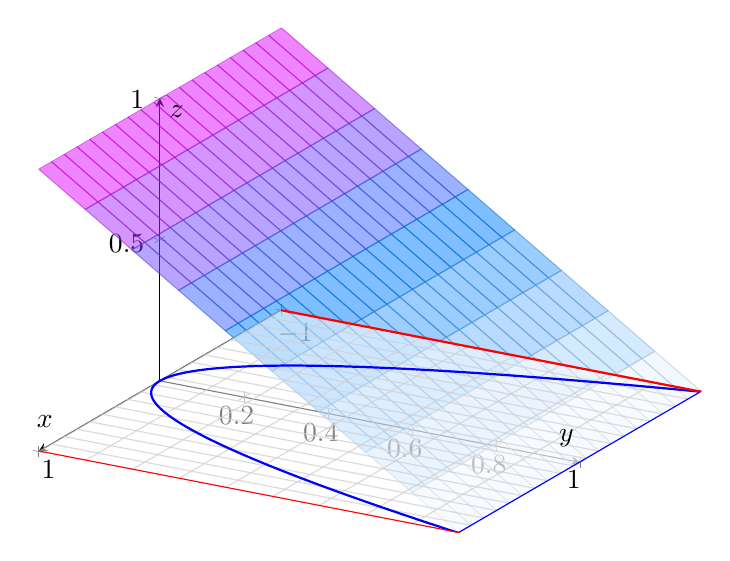
\begin{tikzpicture}
            \begin{axis}[
                    axis lines = middle,
                    xlabel = $x$,
                    ylabel = $y$,
                    zlabel = $z$,
                    domain=-1:1,
                    y domain=0:1,
                    samples=20,
                    samples y=10,
                    colormap/cool,
                    view={120}{30},
                    width=10cm,
                    height=8cm,
                ]
                % Draw the surface z = 1 - y
                \addplot3[surf, opacity=0.5] {1 - y};
                % Draw the plane z = 0
                \addplot3[surf, opacity=0.5] {0};
                % Draw the curve y = x^2
                \addplot3[domain=-1:1, samples=100, thick, blue] ({x}, {x^2}, {0});
                % Draw the vertical lines at x = -1 and x = 1
                \addplot3[domain=0:1, samples=100, thick, red] ({-1}, {x}, {0});
                \addplot3[domain=0:1, samples=100, thick, red] ({1}, {x}, {0});
            \end{axis}
        \end{tikzpicture}
        \caption{The region bounded by $z = 1 - y$, $z = 0$, $y = x^2$, $x = -1$, and $x = 1$.}
    \end{figure}
    
    
    We can also visualize the $R$ that is the reigion projected in the $xy$-plane as follows
    
    \begin{figure}[h!]
        \centering
        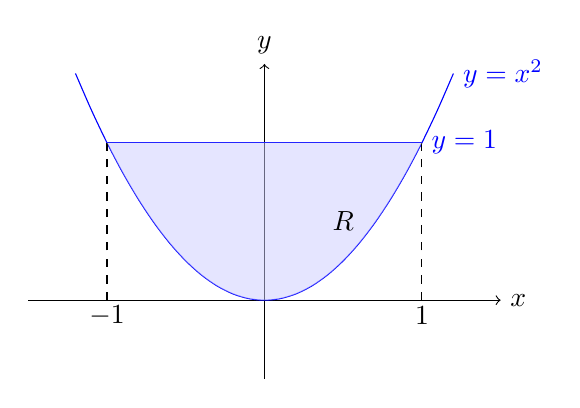
\begin{tikzpicture}[scale=2]
            % Draw axes
            \draw[->] (-1.5,0) -- (1.5,0) node[right] {$x$};
            \draw[->] (0,-0.5) -- (0,1.5) node[above] {$y$};
            
            % Draw the curve y = x^2
            \draw[domain=-1.2:1.2,smooth,variable=\x,blue] plot ({\x},{\x*\x}) node[right] {$y = x^2$};
            % Draw the line y = 1
            \draw[blue] (-1,1) -- (1,1) node[right] {$y = 1$};

            %vertical labels for x = pm1
            \draw[dashed] (-1,0) -- (-1,1);
            \draw[dashed] (1,0) -- (1,1);
            \node at (-1,-0.1) {$-1$};
            \node at (1,-0.1) {$1$};

            % Shade the region
            \fill[blue!20,opacity=0.5] plot[domain=-1:1,smooth,variable=\x] ({\x},{\x*\x}) -- (1,1) -- (-1,1) -- cycle;
            % Add labels
            \node at (0.5,0.5) {$R$};
        \end{tikzpicture}
        \caption{The projection of the region onto the $xy$-plane.}
        
    \end{figure}

    So, we can consider the projection of the triangle on the $zy$-plane as our base region $R'$. Then, we consider how the region changes in the $x$ direction over $R$:
    $$
        x^2 = y \implies -\sqrt{y} \le x \le \sqrt{y}
    $$
    So we can set up:
    \begin{align*}
        \iiint_V f(x,y,z) \, dV &= \iint_{R'} \int_{-\sqrt{y}}^{\sqrt{y}} f(x,y,z) \, dx \, dA \\
        &= \iint_{R'} \int_{-\sqrt{y}}^{\sqrt{y}} f(x,y,z) \, dx \, dy \, dz
    \end{align*}
    Now, we consider how the projection $R'$ change in the $y$ direction over $z$:
    $$        z = 1 - y \implies 0 \le y \le 1 - z, \quad 0 \le z \le 1
    $$
    So we can set up:
    \begin{align*}
        \iiint_V f(x,y,z) \, dV &= \int_0^1 \int_0^{1 - z} \int_{-\sqrt{y}}^{\sqrt{y}} f(x,y,z) \, dx \, dy \, dz
    \end{align*}
\end{example}
\subsubsection{Applications of Triple Integrals}
\paragraph{Physical Applications} Similar to double integrals, triple integrals can be used to compute physical quantities such as mass, center of mass, and moment of inertia for three-dimensional objects with variable density. 
\begin{definition}[Mass of a Solid]
    Consider a solid $V$ with a variable density function $\rho(x,y,z)$ that is continuous over the solid. The mass $M$ of the solid can be computed using the following triple integral:
    \begin{equation}
        M = \iiint_V \rho(x,y,z) \, dV
    \end{equation}
    
\end{definition}

\begin{definition}[Center of Mass of a Solid]
    Consider a solid $V$ with a variable density function $\rho(x,y,z)$ that is continuous over the solid. The coordinates of the center of mass $(\bar{x}, \bar{y}, \bar{z})$ of the solid can be computed using the following formulas:
    \begin{equation}
        \bar{x} = \frac{1}{M} \iiint_V x \rho(x,y,z) \, dV, \quad \bar{y} = \frac{1}{M} \iiint_V y \rho(x,y,z) \, dV, \quad \bar{z} = \frac{1}{M} \iiint_V z \rho(x,y,z) \, dV
    \end{equation}
    where $M$ is the mass of the solid.
    
\end{definition}


\begin{definition}[Moment of Inertia of a Solid]
    Consider a solid $V$ with a variable density function $\rho(x,y,z)$ that is continuous over the solid. The moment of inertia of the solid about the $x$-axis ($I_x$), $y$-axis ($I_y$), and $z$-axis ($I_z$) can be computed using the following formulas:
    \begin{equation}
        I_x = \iiint_V (y^2 + z^2) \rho(x,y,z) \, dV, \quad I_y = \iiint_V (x^2 + z^2) \rho(x,y,z) \, dV, \quad I_z = \iiint_V (x^2 + y^2) \rho(x,y,z) \, dV
    \end{equation}
    where $y^2 + z^2$, $x^2 + z^2$, and $x^2 + y^2$ are the squares of the distances from the respective axes of rotation, and $\rho(x,y,z) \, dV$ represents the mass element of the solid at the point $(x,y,z)$.

    Also for the moment of inertia about the origin ($I_o$):
    \begin{equation}
        I_o = \iiint_V (x^2 + y^2 + z^2) \rho(x,y,z) \, dV
    \end{equation}
    In general, for an axis defined by a line $ax + by + cz + d = 0$, the moment of inertia about that axis ($I_l$) can be found using the following formula:
    \begin{equation}
        I_l = \iiint_V \left( \frac{ax + by + cz + d}{\sqrt{a^2 + b^2 + c^2}} \right)^2 \rho(x,y,z) \, dV
    \end{equation}
\end{definition}

\begin{example}
    \textit{Find the center of mass of a solid of constant density $\rho_0$ that is bounded by the parabolic cylinder $x = y^2$ and the planes $z=0$, $x=z$ and $x=1$.}
    We visualize the solid as follows:
    \begin{figure}[h!]
        \centering
        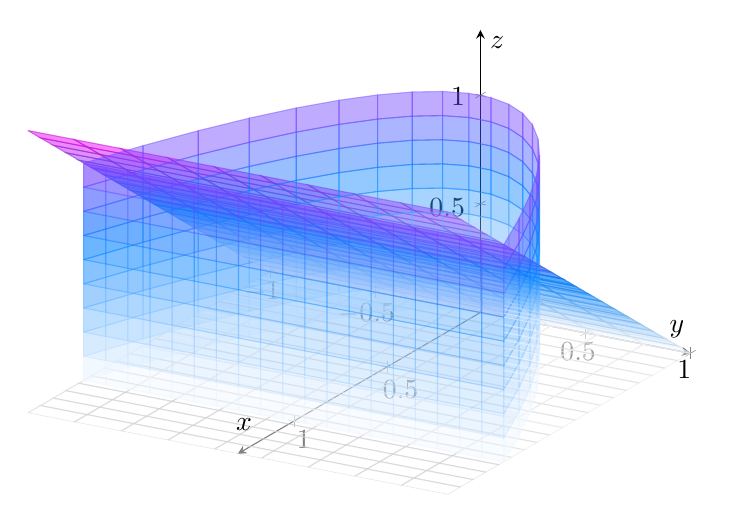
\begin{tikzpicture}
            \begin{axis}[
                    axis lines = middle,
                    xlabel = $x$,
                    ylabel = $y$,
                    zlabel = $z$,
                    domain=0:1.3,
                    y domain=-1:1,
                    samples=20,
                    samples y=10,
                    colormap/cool,
                    view={120}{30},
                    width=10cm,
                    height=8cm,
                ]
                % Draw the surface z = x
                \addplot3[surf, opacity=0.5] {x};
                % Draw the plane z = 0
                \addplot3[surf, opacity=0.5] {0};

                % Draw the surface cylinder x = y^2 on the plane z = 0, and it extends to z = x
                % Parabolic cylinder x = y^2 (y in [-1,1], z in [0,1])
                \addplot3[surf, opacity=0.45, shader=flat, domain=-1:1, y domain=0:1] ({x^2}, {x}, {y});
                % bottom z = 0
                \addplot3[surf, opacity=0.25, shader=flat, domain=0:1, y domain=-1:1] ({x}, {y}, {0});
                % slanted plane x = z (i.e. z = x)
                \addplot3[surf, opacity=0.35, shader=flat, domain=0:1, y domain=-1:1] ({x}, {y}, {x});
                % vertical plane x = 1 (closes the solid)
                \addplot3[surf, opacity=0.30, shader=flat, domain=-1:1, y domain=0:1] ({1}, {x}, {y});
                % fill the surface such that
            \end{axis}
        \end{tikzpicture}
        \caption{The solid bounded by the surfaces $x = y^2$, $z = 0$, $x = z$, and $x = 1$.}
    \end{figure}
    We can find the mass of the solid:
    \begin{align*}
        M &= \iiint_V \rho_0 \, dV = \rho_0 \iiint_V 1 \, dV \\
        &= \rho_0 \int_{-1}^1 \int_{y^2}^1 \int_{0}^x 1 \, dz \, dx \, dy \\
        &= \rho_0 \cdot \frac{4}{5}
    \end{align*}

    Next, we can find the coordinates of the center of mass:
    \begin{align*}
        \bar{x} &= \frac{1}{M} \iiint_V x \rho_0 \, dV = \frac{\rho_0}{M} \iiint_V x \, dV = 5/7 \\
        \bar{y} &= \frac{1}{M} \iiint_V y \rho_0 \, dV = \frac{\rho_0}{M} \iiint_V y \, dV = 0 \text{ (by symmetry)} \\
        \bar{z} &= \frac{1}{M} \iiint_V z \rho_0 \, dV = \frac{\rho_0}{M} \iiint_V z \, dV = 5/14 \\
    \end{align*}    
\end{example}

\begin{example}
    \textit{Find the moment of inertia of a cyliner with radius $a$ and height $h$ about its central axis, assuming the cylinder has a constant density $\rho_0$.}
    We consider the base region $R$ as the circular base of the cylinder in the $xy$-plane. Then, we consider how the cylinder change in the $z$ direction over $R$:
    $$
        0 \le z \le h
    $$
    So we can set up:
    \begin{align*}
        I_z &= \iiint_V (x^2 + y^2) \rho_0 \, dV = \rho_0 \iint_R \int_0^h (x^2 + y^2) \, dz \, dA \\
        &= \rho_0 h \iint_R (x^2 + y^2) \, dA
    \end{align*}

    Then, we can express the base region $R$ in polar coordinates:
    $$        
    x^2 + y^2 = r^2 \implies 0 \le r \le a, \quad 0 \le \theta \le 2\pi
    $$
    So we can set up:
    \begin{align*}
        I_z &= \rho_0 h \int_0^{2\pi} \int_0^a r^2 \cdot r \, dr \, d\theta \\
        &= \rho_0 h \int_0^{2\pi} \left[ \frac{r^4}{4} \right]_{r=0}^{r=a} \, d\theta = \frac{\pi \rho_0 h a^4}{2}
    \end{align*}
    This also leads to the well-known formula for the moment of inertia of a solid cylinder about its central axis:
    $$
        I_z = \frac{1}{2} M a^2
    $$
    where $M = \pi a^2 h \rho_0$ is the mass of the cylinder. 
\end{example}
\subsection{Triple Integrals in Cylindrical Coordinates}

\begin{keybox}
	\textbf{Key Relations:}
\begin{itemize}
    \item $(r,\theta,z)$ with $x=r\cos\theta$, $y=r\sin\theta$, $dV=r\,dr\,d\theta\,dz$.
    \item Use when symmetry around $z$-axis or $x^2{+}y^2$ appears.
\end{itemize}
	\textbf{Tip:} Don’t forget the Jacobian factor $r$.
\end{keybox}
\begin{definition}[Cylindrical Coordinates]
    The cylindrical coordinates of a point $P$ in 3-D space are given by the ordered triple $(r, \theta, z)$, where:
    \begin{itemize}
        \item $r$ is the distance from the $z$-axis to the projection of $P$ onto the $xy$-plane,
        \item $\theta$ is the angle between the positive $x$-axis and the line segment from the origin to the projection of $P$ onto the $xy$-plane,
        \item $z$ is the same as in rectangular coordinates, representing the height of point $P$ above the $xy$-plane.
    \end{itemize}
    The relationships between cylindrical coordinates and rectangular coordinates are given by:
    \begin{equation}
        x = r \cos \theta, \quad y = r \sin \theta, \quad z = z
    \end{equation}
    and conversely:
    \begin{equation}
        r = \sqrt{x^2 + y^2}, \quad \theta = \tan^{-1}\left(\frac{y}{x}\right), \quad z = z
    \end{equation}

    For the change of variables in triple integrals, the volume element $dV$ in cylindrical coordinates is given by:
    \begin{equation}
        dV = dA \, dz = r \, dr \, d\theta \, dz
    \end{equation}
\end{definition}

\begin{example}
    Consider the triple integral in the cononical reigion $V$ bounded by the cone $z = \sqrt{x^2 + y^2}$ and the plane $z=2$. Changing to cylindrical coordinates, we consider the projection of the cone onto the $xy$-plane as our polar base region $R$. Then, we consider how the cone change in the $z$ direction over $R$:
    $$
        z = r \implies r \le z \le 2
    $$
    So the region $V_{\text{polar}}$ is:
    $$
    V_{\text{polar}} = \{(r, \theta, z) \mid 0 \le r \le 2, 0 \le \theta \le 2\pi, r \le z \le 2\}
    $$
    So we can set up:
    $$
        \iiint_V f(x,y,z) \, dV = \int_0^{2\pi} \int_0^2 \int_r^2 f(r \cos \theta, r \sin \theta, z) \, r \, dz \, dr \, d\theta
    $$

    Let $f(x,y,z) = x^2 +. y^2 = r^2$. Then, we have:
    \begin{align*}
        \iiint_V (x^2 + y^2) \, dV &= \int_0^{2\pi} \int_0^2 \int_r^2 r^2 \cdot r \, dz \, dr \, d\theta \\
        &= \int_0^{2\pi} \int_0^2 r^3 (2 - r) \, dr \, d\theta = \frac{16\pi}{5}
    \end{align*}

\end{example}
\subsection{Triple Integrals in Spherical Coordinates}

\begin{keybox}
	\textbf{Key Relations:}
\begin{itemize}
    \item $(\rho,\phi,\theta)$ with $x=\rho\sin\phi\cos\theta$, $y=\rho\sin\phi\sin\theta$, $z=\rho\cos\phi$.
    \item $dV=\rho^2\sin\phi\,d\rho\,d\phi\,d\theta$.
\end{itemize}
	\textbf{Tips:}
\begin{itemize}
    \item Spheres/cones/spherical caps are natural in these coordinates.
    \item Bound order: typically $\rho$ (inner), then $\phi$, then $\theta$.
\end{itemize}
\end{keybox}
\begin{definition}[Spherical Coordinates]
    The spherical coordinates of a point $P$ in 3-D space are given by the ordered triple $(\rho, \phi, \theta)$, where:
    \begin{itemize}
        \item $\rho$ is the distance from the origin to the point $P$,
        \item $\phi$ is the angle between the positive $z$-axis and the line segment from the origin to point $P$ (also known as the polar angle or colatitude),
        \item $\theta$ is the angle between the positive $x$-axis and the projection of the line segment from the origin to point $P$ onto the $xy$-plane (also known as the azimuthal angle).
    \end{itemize}
    The relationships between spherical coordinates and rectangular coordinates are given by:
    \begin{equation}
        x = \rho \sin \phi \cos \theta, \quad y = \rho \sin \phi \sin \theta, \quad z = \rho \cos \phi
    \end{equation}
    and conversely:
    \begin{equation}
        \rho = \sqrt{x^2 + y^2 + z^2}, \quad \phi = \cos^{-1}\left(\frac{z}{\sqrt{x^2 + y^2 + z^2}}\right), \quad \theta = \tan^{-1}\left(\frac{y}{x}\right)
    \end{equation}

    For the change of variables in triple integrals, the volume element $dV$ in spherical coordinates is given by:
    \begin{equation}
        dV = \rho^2 \sin \phi \, d\rho \, d\phi \, d\theta
    \end{equation}
\end{definition}

\begin{example}
    \textit{find the mass of a half sphere of radius $a$ that has a density $ k(2a - \rho)$, where $k$ is a constant and $\rho$ is the distance from the origin.}

    Let $\lambda = k(2a - \rho)$ be the density function. Then, we consider the half sphere $S$ in spherical coordinates:
    $$       
    S = \{(\rho, \phi, \theta) \mid 0 \le \rho \le a, 0 \le \phi \le \frac{\pi}{2}, 0 \le \theta \le 2\pi\}
    $$
    So we can set up:
    \begin{align*}
        M &= \iiint_S \lambda \, dV = \iiint_S k(2a - \rho) \, dV \\
        &= k \int_0^{2\pi} \int_0^{\frac{\pi}{2}} \int_0^a (2a - \rho) \rho^2 \sin \phi \, d\rho \, d\phi \, d\theta \\
        &= k \int_0^{2\pi} \int_0^{\frac{\pi}{2}} \left[ 2a \cdot \frac{\rho^3}{3} - \frac{\rho^4}{4} \right]_{\rho=0}^{\rho=a} \sin \phi \, d\phi \, d\theta \\
        &= k \int_0^{2\pi} \int_0^{\frac{\pi}{2}} \left( \frac{2a^4}{3} - \frac{a^4}{4} \right) \sin \phi \, d\phi \, d\theta \\
        &= k \cdot \frac{5a^4}{12} \int_0^{2\pi} \left[ -\cos \phi \right]_{\phi=0}^{\phi=\frac{\pi}{2}} \, d\theta = k \cdot \frac{5a^4}{12} \cdot 2\pi \\ 
        &= \frac{5\pi k a^4}{6}
    \end{align*}

\end{example}
\subsection{Change of Variables in Multiple Integrals} \label{sec:change_of_variables}

\begin{keybox}
	\textbf{Key Equations:}
\begin{itemize}
    \item $\displaystyle \iint_R f(x,y)\,dA = \iint_{R'} f(x(u,v),y(u,v))\,\left|\det J\right|\,du\,dv$.
    \item $J=\partial(x,y)/\partial(u,v)$; similarly for 3D.
\end{itemize}
	\textbf{Tips/Pitfalls:}
\begin{itemize}
    \item Map the region carefully; sketch both $R$ and $R'$.
    \item Include the Jacobian; watch sign via absolute value.
\end{itemize}
\end{keybox}
\begin{shaded}
    \subsubsection{Change of Variables in Single Integrals}
    Consider the following integral:
    $$
        \int_1^3 2x\sqrt{x^2 +1} \, dx
    $$
    We can use substitution to solve this integral. Let $u = x^2 + 1$, then $du = 2x \, dx$. Then, we carefully plug in to the integral, and notice how this could extend to multiple integrals:
    \begin{align*}
        \int_1^3 2x\sqrt{x^2 +1} \, dx &= \int_{u=2}^{u=10} 2 \sqrt{u} \sqrt{u-1} \cdot \frac{du}{2\sqrt{u-1}} = \int_{u=2}^{u=10} \sqrt{u} \, du \\
        &= \left[ \frac{2}{3} u^{\frac{3}{2}} \right]_{u=2}^{u=10} = \frac{2}{3} (10^{\frac{3}{2}} - 2^{\frac{3}{2}})
    \end{align*}
    The key step is to express $dx$ in terms of $du$:
    $$        
    dx = \frac{du}{2x}
    $$
    Consider how the area under a curve shifts when we change the variable from $x$ to $u$, we can visualize this as follows:
    % two minipages side by side one with the graph of y = f(x) from 0 to 3 and the other with the graph of y = f(u) from 2 to 10
    \end{shaded}
    \newpage

    \begin{figure}[h!]
        \centering
        \begin{minipage}{0.45\textwidth}
            \centering
            \begin{tikzpicture}
                \begin{axis}[
                        axis lines = middle,
                        xlabel = $x$,
                        ylabel = $y$,
                        domain=0:3,
                        samples=100,
                        width=6cm,
                        height=5cm,
                    ]
                    % Draw the curve y = f(x) and name the x-axis as a path
                    \addplot[blue, thick, name path=fcurve] {2*x*sqrt(x^2 + 1)};
                    \addplot[thick, name path=axisline] {0};
                    % Draw vertical guide lines (for visual reference)
                    \draw[black, thick] (axis cs:1,0) -- (axis cs:1,8);
                    \draw[black, thick] (axis cs:3,0) -- (axis cs:3,18);
                    % Shade the area under the curve from x=1 to x=3 using fill between curve and axis
                    \addplot[blue!20, opacity=0.5] fill between[of=fcurve and axisline, soft clip={domain=1:3}];
                    % Add labels
                    \node at (axis cs:2,5) {$y = f(x)$};
                    \node at (axis cs:2,1) {Area};
                \end{axis}
            \end{tikzpicture}
            \caption{Area under the curve $y = f(x)$ from $x=1$ to $x=3$.}
        \end{minipage}
        \hfill
        \begin{minipage}{0.45\textwidth}
            \centering
            \begin{tikzpicture}
                \begin{axis}[
                        axis lines = middle,
                        xlabel = $u$,
                        ylabel = $y$,
                        domain=0:12,
                        samples=100,
                        width=6cm,
                        height=5cm,
                    ]
                    % Draw the curve y = f(u) and name the x-axis as a path
                    \addplot[blue, thick, name path=gcurve] {2*sqrt(x)*sqrt(x - 1)};
                    \addplot[thick, name path=axisline] {0};
                    % Shade the area under the curve from u=2 to u=10 using fill between curve and axis
                    \addplot[blue!20, opacity=0.5] fill between[of=gcurve and axisline, soft clip={domain=2:10}];
                    % Add labels
                    \node at (axis cs:6,9) {$y = f(u)$};
                    \node at (axis cs:6,3) {Area};
                \end{axis}
            \end{tikzpicture}
            \caption{Area under the curve $y = f(u)$ from $u=2$ to $u=10$.}
        \end{minipage}  
    \end{figure}
\begin{shaded}

    Although $2x \sqrt{x^2 + 1} = 2\sqrt{u} \sqrt{u-1}$, the area under the curve at any given $x_0$, $u_0 = x_0^2 + 1$ are not necessarily equal: $f(x_0) \neq f(u_0)$. This is because the width of each rectangle changes when we change the variable from $x$ to $u$. But for small changes, we can approximate the width of each rectangle as follows:
    $$        
    \Delta u \approx \frac{du}{dx} \Delta x = 2x \Delta x
    $$
    So, the area of each rectangle changes as follows:
    $$        
    \text{Area} \approx f(x) \Delta x = f(u) \frac{\Delta u}{2x}
    $$
    Taking the limit as $\Delta x \to 0$ (and thus $\Delta u \to 0$), we get:
    $$        
    \text{Area} = f(x) \, dx = f(u) \frac{du}{2x}
    $$
    This is the key idea behind the change of variables in integrals, and it can be extended to multiple integrals.
\end{shaded}

\paragraph{Change of Variables in Double Integrals} Consider the following change of variables in double integral $\iint_R f(x,y) \, dA$:
$$
\begin{cases}
    x = g(u,v) \\
    y = h(u,v)
\end{cases}
$$
Such that we call the corresponding region in the $uv$-plane as $S$. Now we assume that there exists a bijective mapping between $(x,y)$ and $(u,v)$, and that the functions $g$ and $h$ have continuous partial derivatives. Then, we can express the area element $dA$ in terms of $du$ and $dv$.

We can imagine any uniform small rectangle in the $uv$-plane with sides $\Delta u$ and $\Delta v$. Consider how the four corners of the rectangle map to the $xy$-plane:
\begin{itemize}
    \item The corner at $(u,v)$ maps to $(x,y) = (g(u,v), h(u,v))$.
    \item The corner at $(u + \Delta u, v)$ maps to $(x,y) = (g(u + \Delta u, v), h(u + \Delta u, v))$.
    \item The corner at $(u, v + \Delta v)$ maps to $(x,y) = (g(u, v + \Delta v), h(u, v + \Delta v))$.\end{itemize}
And we can consider the infinitesimal case as $\Delta u \to 0$ and $\Delta v \to 0$. Then, we can approximate the area of the parallelogram (we can prove this is a parallelogram as the dot product of the two sides converge to 0) formed by these four points in the $xy$-plane by the magnitude of the cross product of the two vectors. 

First, we consider the first order taylor approximateion of $g$ and $h$ at the above four corners:
\begin{align*}
    g(u + \Delta u, v) &\approx g(u,v) + g_u(u,v) \Delta u \\
    h(u + \Delta u, v) &\approx h(u,v) + h_u(u,v) \Delta u \\
    g(u, v + \Delta v) &\approx g(u,v) + g_v(u,v) \Delta v \\
    h(u, v + \Delta v) &\approx h(u,v) + h_v(u,v) \Delta v \\
\end{align*}
And then we condsier the vecotr's form of the two sides of the parallelogram:
\begin{align*}
    \overrightarrow{A} &= \langle g(u + \Delta u, v) - g(u,v), h(u + \Delta u, v) - h(u,v) \rangle \\
    &\approx \Delta u \langle g_u(u,v), h_u(u,v) \rangle \\
    \overrightarrow{B} &= \langle g(u, v + \Delta v) - g(u,v), h(u, v + \Delta v) - h(u,v) \rangle \\
    &\approx \Delta v \langle g_v(u,v), h_v(u,v) \rangle
\end{align*}
Now, we can compute the area of the parallelogram as follows:
\begin{align*}
    \text{Area} &\approx |\overrightarrow{A} \times \overrightarrow{B}| = \left| \begin{vmatrix}
        \mathbf{i} & \mathbf{j} & \mathbf{k} \\
        g_u(u,v) \Delta u & h_u(u,v) \Delta u & 0 \\
        g_v(u,v) \Delta v & h_v(u,v) \Delta v & 0
    \end{vmatrix} \right| \\
    &= \left| (0 - 0) \mathbf{i} - (0 - 0) \mathbf{j} + (g_u(u,v) h_v(u,v) - g_v(u,v) h_u(u,v)) \Delta u \Delta v \mathbf{k} \right| \\
    &= |g_u(u,v) h_v(u,v) - g_v(u,v) h_u(u,v)| \Delta u \Delta v
\end{align*}
Taking the limit as $\Delta u \to 0$ and $\Delta v \to 0$, we get:
$$
dA = |g_u(u,v) h_v(u,v) - g_v(u,v) h_u(u,v)| \, du \, dv
$$
which could be rewritten as the following defintion:

\begin{definition}[Jacobian of a Transformation]
    Consider the transformation:
    $$
    \begin{cases}
        x = g(u,v) \\
        y = h(u,v)
    \end{cases}
    $$
    The Jacobian of the transformation is defined as:
    \begin{equation}
        J = \left| \frac{\partial(x,y)}{\partial(u,v)} \right|= \begin{vmatrix}
            \dfrac{\partial x}{\partial u} & \dfrac{\partial x}{\partial v} \\
            \dfrac{\partial y}{\partial u} & \dfrac{\partial y}{\partial v}
        \end{vmatrix} = g_u(u,v) h_v(u,v) - g_v(u,v) h_u(u,v)
        \end{equation}
    And the area element $dA$ in terms of $du$ and $dv$ is given by:
    $$
        dA = |J| \, du \, dv
    $$
    Additionally, we if we define the chang of variable the other way around:
    $$
    \begin{cases}
        u = p(x,y) \\
        v = q(x,y)
    \end{cases}
    $$
    Then, the Jacobian of the transformation is defined as:
    $$
        J = \frac{\partial(u,v)}{\partial(x,y)} = \begin{vmatrix}
            \dfrac{\partial u}{\partial x} & \dfrac{\partial u}{\partial y} \\
            \dfrac{\partial v}{\partial x} & \dfrac{\partial v}{\partial y}
        \end{vmatrix} = p_x(x,y) q_y(x,y) - p_y(x,y) q_x(x,y)
    $$
    And the area element $dA$ in terms of $dx$ and $dy$ is given by:
    $$        
        dA = \frac{1}{|J|} \, dx \, dy
    $$
    
    WLOG, the Jacobian can be defined for any number of variables. The geneal Jacobian for a transformation is defined as:
    \begin{equation}
        J = \frac{\partial(x_1, x_2, \ldots, x_n)}{\partial(u_1, u_2, \ldots, u_n)} = \begin{vmatrix}
            \dfrac{\partial x_1}{\partial u_1} & \dfrac{\partial x_1}{\partial u_2} & \cdots & \dfrac{\partial x_1}{\partial u_n} \\
            \dfrac{\partial x_2}{\partial u_1} & \dfrac{\partial x_2}{\partial u_2} & \cdots & \dfrac{\partial x_2}{\partial u_n} \\
            \vdots & \vdots & \ddots & \vdots \\
            \dfrac{\partial x_n}{\partial u_1} & \dfrac{\partial x_n}{\partial u_2} & \cdots & \dfrac{\partial x_n}{\partial u_n}
        \end{vmatrix}
    \end{equation}
    for the transformation:
    $$
    \begin{cases}
        x_1 = g_1(u_1, u_2, \ldots, u_n) \\
        x_2 = g_2(u_1, u_2, \ldots, u_n) \\
        \vdots \\
        x_n = g_n(u_1, u_2, \ldots, u_n)
    \end{cases}
    $$
\end{definition}

\begin{example}[Change to Polar Coordinates]
    Consider the change of variables from rectangular coordinates $(x,y)$ to polar coordinates $(r,\theta)$:
    $$
    \begin{cases}
        x = r \cos \theta \\
        y = r \sin \theta
    \end{cases}
    $$
    We can compute the Jacobian of this transformation as follows:
    \begin{align*}
        J &= \frac{\partial(x,y)}{\partial(r,\theta)} = \begin{vmatrix}
            \dfrac{\partial x}{\partial r} & \dfrac{\partial x}{\partial \theta} \\
            \dfrac{\partial y}{\partial r} & \dfrac{\partial y}{\partial \theta}
        \end{vmatrix} = \begin{vmatrix}
            \cos \theta & -r \sin \theta \\
            \sin \theta & r \cos \theta
        \end{vmatrix} \\
        &= r (\cos^2 \theta + \sin^2 \theta) = r
    \end{align*}
    So, the area element $dA$ in terms of $dr$ and $d\theta$ is given by:
    $$        
        dA = |J| \, dr \, d\theta = r \, dr \, d\theta
    $$
    This is consistent with the formula for the area element in polar coordinates.
\end{example}

\begin{example}
    Cosndier the interal:
    $$
        \iint_R (x^2 + 2xy) \, dA
    $$
    where $R$ the region bounded by the lines $y=2x + 3$ and $y=2x + 1$, $y=5-x$ and $y=2 - x$.

    Motivated by the bounds, we can use the change of variables:
    $$
    \begin{cases}
        u = y - 2x \\
        v = y + x
    \end{cases}
    $$ 
    So, let $S$ be the corresponding region in the $uv$-plane. We can find the bounds of $S$ by plugging in the lines that bound $R$:
    \begin{itemize}
        \item $y = 2x + 3 \implies u = 3$
        \item $y = 2x + 1 \implies u = 1$
        \item $y = 5 - x \implies v = 5$
        \item $y = 2 - x \implies v = 2$
    \end{itemize}
    
    Then, we consider the Jacobian. First, we express $x$ and $y$ in terms of $u$ and $v$:
    $$
    \begin{cases}
        u = y - 2x \\
        v = x + y
    \end{cases} \implies \begin{cases}
        x = \frac{1}{3} (v - u) \\
        y = \frac{1}{3} (2v + u)
    \end{cases}
    $$
    Then, we can compute the Jacobian of this transformation as follows:
    \begin{align*}
        J &= \frac{\partial(x,y)}{\partial(u,v)} = \begin{vmatrix}
            \dfrac{\partial x}{\partial u} & \dfrac{\partial x}{\partial v} \\
            \dfrac{\partial y}{\partial u} & \dfrac{\partial y}{\partial v}
        \end{vmatrix} = \begin{vmatrix}
            -\frac{1}{3} & \frac{1}{3} \\
            \frac{1}{3} & \frac{2}{3}
        \end{vmatrix} \\
        &= -\frac{2}{9} - \frac{1}{9} = -\frac{1}{3}
    \end{align*}
    So, we can express the integral in terms of $u$ and $v$:
    \begin{align*}
        \iint_R (x^2 + 2xy) \, dA &= \iint_S \left( \left(\frac{1}{3} (v - u)\right)^2 + 2 \cdot \frac{1}{3} (v - u) \cdot \frac{1}{3} (2v + u) \right) |J| \, du \, dv \\
        &= \iint_S \left( \frac{1}{9} (v - u)^2 + \frac{2}{9} (v - u)(2v + u) \right) \cdot \frac{1}{3} \, du \, dv \\
        &= \frac{1}{27} \iint_S (5v^2 - u^2) \, du \, dv \\
        &= \frac{196}{27}
    \end{align*}
\end{example}

\begin{example} \label{ex:change_of_variables}
    \textit{Evaluate the integral}
    $$
        \iint_R xy \, dA
    $$
    where $R$ is the region bounded by curves $x^2 + y^2 = 4$, $x^2 + y^2 = 9$, $x^2 - y^2 = 1$, and $x^2 - y^2 = 4$.

    Motivated by the bounds, we can use the change of variables:
    $$
    \begin{cases}
        u = x^2 + y^2 \\
        v = x^2 - y^2
    \end{cases} \implies \begin{cases}
        x = \sqrt{\frac{u + v}{2}} \\
        y = \sqrt{\frac{u - v}{2}}
    \end{cases}
    $$
    The jacobian of this transformation is:
    \begin{align*}
        J &= \frac{\partial(x,y)}{\partial(u,v)} = \begin{vmatrix}
            \dfrac{\partial x}{\partial u} & \dfrac{\partial x}{\partial v} \\
            \dfrac{\partial y}{\partial u} & \dfrac{\partial y}{\partial v}
        \end{vmatrix} = \begin{vmatrix}
            \frac{1}{2\sqrt{2(u+v)}} & \frac{1}{2\sqrt{2(u+v)}} \\
            \frac{1}{2\sqrt{2(u-v)}} & -\frac{1}{2\sqrt{2(u-v)}}
        \end{vmatrix} \\
        &= -\frac{1}{8} \left( \frac{1}{\sqrt{u^2 - v^2}} + \frac{1}{\sqrt{u^2 - v^2}} \right) = -\frac{1}{4\sqrt{u^2 - v^2}}
    \end{align*}
    So, we can express the integral in terms of $u$ and $v$:
    \begin{align*}
        \iint_R xy \, dA &= \iint_S \sqrt{\frac{u + v}{2}} \cdot \sqrt{\frac{u - v}{2}} \cdot |J| \, du \, dv \\
        &= \iint_S \frac{\sqrt{u^2 - v^2}}{2} \cdot \frac{1}{4\sqrt{u^2 - v^2}} \, du \, dv = \iint_S \frac{1}{8} \, du \, dv \\
        &= \int_1^4 \int_4^9 \frac{1}{8} \, dv \, du = \frac{1}{8}(4 - 1)(9 - 4) = \frac{15}{8}
    \end{align*}
    
\end{example}

\begin{theorem}[Back Transformation]
    Consider the Jacobian $J$ of a transformation:
    $$
    \begin{cases}
        x = g(u,v) \\
        y = h(u,v)
    \end{cases}
    $$
    If $J \neq 0$, then the Jacobian of the inverse transformation:
    $$
    \begin{cases}
        u = p(x,y) \\
        v = q(x,y)
    \end{cases}
    $$
    is given by:
    \begin{equation}
        J^{-1} = \frac{\partial(u,v)}{\partial(x,y)} = \frac{1}{\frac{\partial(x,y)}{\partial(u,v)}}
    \end{equation}
\end{theorem}
\begin{proof}
    % a short intuitive proof sketch
    \textbf{Sketch:} Consider a small rectangle in the $uv$-plane with sides $\Delta u$ and $\Delta v$. The area of this rectangle is $\Delta A_{uv} = \Delta u \Delta v$. This rectangle maps to a parallelogram in the $xy$-plane with area $\Delta A_{xy} \approx |J| \Delta u \Delta v$. Now, consider the inverse transformation. A small rectangle in the $xy$-plane with sides $\Delta x$ and $\Delta y$ maps back to a parallelogram in the $uv$-plane with area $\Delta A_{uv} \approx |J^{-1}| \Delta x \Delta y$. Since these areas must be consistent under the transformations, we have:
    $$
        |J| \Delta u \Delta v = \Delta x \Delta y \quad \text{and} \quad |J^{-1}| \Delta x \Delta y = \Delta u \Delta v
    $$
    Dividing the first equation by the second, we get:
    $$
        |J| = \frac{1}{|J^{-1}|}
    $$
\end{proof}

\begin{example}
    Consider the transformation and integral in \ref{ex:change_of_variables}. We can verify the result using the back transformation theorem. The Jacobian of the inverse transformation is:
    \begin{align*}
        J^{-1} &= \frac{\partial(u,v)}{\partial(x,y)} = \begin{vmatrix}
            \dfrac{\partial u}{\partial x} & \dfrac{\partial u}{\partial y} \\
            \dfrac{\partial v}{\partial x} & \dfrac{\partial v}{\partial y}
        \end{vmatrix} = \begin{vmatrix}
            2x & 2y \\
            2x & -2y
        \end{vmatrix} \\
        &= -4xy - 4xy = -8xy
    \end{align*}
    So, we have:
    $$        
        J = \frac{1}{J^{-1}} = -\frac{1}{8xy} \implies I = \iint_R xy \, dA = \iint_S \frac{xy}{8xy} \, du \, dv = \iint_S \frac{1}{8} \, du \, dv = \frac{15}{8}
    $$
    This is consistent with the result we obtained in \ref{ex:change_of_variables}, and results in a much simpler integral to evaluate.
\end{example}

\begin{example}
    Consider the integral:  
    $$
        \iint_R \exp{\left(\frac{x - y}{x + y}\right)} \, dA
    $$
    where $R$ is the trapezoid with vertices at $(1,0)$, $(2,0)$, $(0,-2)$ and $(0,-1)$.

    Motivated by the integrabled, we can use the change of variables:
    $$
    \begin{cases}
        u = x + y \\
        v = x - y
    \end{cases} 
    $$
    Also, we can define our bounds as follow:
    \begin{itemize}
        \item $y = x - 2 \implies u = 2$
        \item $y = x - 1 \implies v = 1$
        \item $x = 0 \implies u = -v$
        \item $y = 0 \implies u = v$
    \end{itemize}
    We can find the Jacobian of this transformation by its inverse:
    $$
    J^{-1} = \frac{\partial(u,v)}{\partial(x,y)} = \begin{vmatrix}
        \dfrac{\partial u}{\partial x} & \dfrac{\partial u}{\partial y} \\
        \dfrac{\partial v}{\partial x} & \dfrac{\partial v}{\partial y}
    \end{vmatrix} = \begin{vmatrix}
        1 & 1 \\
        1 & -1
    \end{vmatrix} = -2 \implies J = -\frac{1}{2}
    $$
    So, we can write the integral in terms of $u$ and $v$:
    \begin{align*}
        \iint_R \exp{\left(\frac{x - y}{x + y}\right)} \, dA &= \iint_S \exp{\left(\frac{v}{u}\right)} \cdot |J| \, du \, dv \\
        &= \frac{1}{2} \int_1^2 \int_{-v}^{v} \exp{\left(\frac{v}{u}\right)} \, du \, dv \\
        &= \frac{1}{2} \int_1^2 v(e - e^{-1}) \, dv = \frac{3}{4} (e - e^{-1})
    \end{align*}
\end{example}

\begin{example}
    \textit{Evaluate the integral}
    $$
        \iint_R (x^2 - y^2) \exp(xy) \, dA
    $$
    where $R$ is the region bounded by the hyperbolas $xy=1$ and $xy=4$, and the lines $y=x$ and $y=x+2$.

    Motivated by the bounds, we can use the change of variables:
    $$
    \begin{cases}
        u = xy \\
        v = y - x
    \end{cases}
    $$
    So, let $S$ be the corresponding region in the $uv$-plane. We can find the bounds of $S$ by plugging in the lines that bound $R$:   
    \begin{itemize}
        \item $xy = 1 \implies u = 1$
        \item $xy = 4 \implies u = 4$
        \item $y = x \implies v = 0$
        \item $y = x + 2 \implies v = 2$
    \end{itemize}
    We find the Jacobian of this transformation by its inverse:
    $$
    J^{-1} = \frac{\partial(u,v)}{\partial(x,y)} = \begin{vmatrix}
        \dfrac{\partial u}{\partial x} & \dfrac{\partial u}{\partial y} \\
        \dfrac{\partial v}{\partial x} & \dfrac{\partial v}{\partial y}
    \end{vmatrix} = \begin{vmatrix}
        y & x \\
        -1 & 1
    \end{vmatrix} = y + x \implies J = \frac{1}{y + x}
    $$
    So, we can express the integral in terms of $u$ and $v$:
    \begin{align*}
        \iint_R (x^2 - y^2) \exp(xy) \, dA &= \iint_S (x+y)(x-y)e^u \cdot |J| \, du \, dv \\
        &= \int_0^2 \int_1^4 -v e^u \, du \, dv = \int_0^2 -v(e^4 - e) \, dv = 2(e - e^4)
    \end{align*}
\end{example}
\begin{example}
    \textit{Find the volume of the region bounded by the hyperbolic cylinders:}
    $$ 
    xy = 1, \quad xy = 3, \quad xz = 1, \quad xz = 3, \quad x = 36, \quad y = 25, \quad yz = 49
    $$
    Motivated by the bounds, we can use the change of variables:
    $$
    \begin{cases}
        u = xy \\
        v = xz \\
        w = yz
    \end{cases} 
    $$
    So, let $S$ be the corresponding region in the $uvw$-space. We can find the bounds of $S$ by plugging in the surfaces that bound the region:

    \begin{align*}
        1 &\leq u \leq 3 \\
        1 &\leq v \leq 3 \\
        25 &\leq w \leq 49
    \end{align*}

    We find the Jacobian of this transformation by its inverse:
    $$
    J^{-1} = \frac{\partial(u,v,w)}{\partial(x,y,z)} = \begin{vmatrix}
        \dfrac{\partial u}{\partial x} & \dfrac{\partial u}{\partial y} & \dfrac{\partial u}{\partial z} \\
        \dfrac{\partial v}{\partial x} & \dfrac{\partial v}{\partial y} & \dfrac{\partial v}{\partial z} \\
        \dfrac{\partial w}{\partial x} & \dfrac{\partial w}{\partial y} & \dfrac{\partial w}{\partial z}
    \end{vmatrix} = \begin{vmatrix}
        y & x & 0 \\
        z & 0 & x \\
        0 & z & y
    \end{vmatrix} = xyz
    $$
    So, we can express the volume of the region in terms of $u$, $v$ and $w$:
    \begin{align*}
        V &= \iiint_R 1 \, dV = \iiint_S |J| \, du \, dv \, dw = \iiint_S \frac{1}{xyz} \, du \, dv \, dw \\
        &= \int_{25}^{49} \int_1^3 \int_1^3 \frac{1}{\sqrt{\frac{uvw}{y^2}}} \, du \, dv \, dw = \int_{25}^{49} \int_1^3 \int_1^3 \frac{y}{\sqrt{uvw}} \, du \, dv \, dw \\
        &= \int_{25}^{49} \int_1^3 \int_1^3 \frac{5}{\sqrt{uvw}} \, du \, dv \, dw = 5 \int_{25}^{49} \int_1^3 \left[ 2\sqrt{u} \right]_{u=1}^{u=3} \frac{1}{\sqrt{vw}} \, dv \, dw \\
        &= 10(\sqrt{3} - 1) \int_{25}^{49} \left[ 2\sqrt{v} \right]_{v=1}^{v=3} \frac{1}{\sqrt{w}} \, dw = 20(\sqrt{3} - 1)(\sqrt{3} - 1) \int_{25}^{49} \frac{1}{\sqrt{w}} \, dw \\
        &= 20(\sqrt{3} - 1)^2 \left[ 2\sqrt{w} \right]_{w=25}^{w=49} = 40(\sqrt{3} - 1)^2 (7 - 5) = 80(\sqrt{3} - 1)^2
    \end{align*}

\end{example}

\section{Vector Calculus}

\subsection{Line Integrals and Vector Fields}

\begin{keybox}
	\textbf{Key Equations:}
\begin{itemize}
    \item Scalar field: $\displaystyle \int_C f\,ds = \int_a^b f(\mathbf r(t))\,\lVert \mathbf r'(t)\rVert\,dt$.
    \item Vector field work: $\displaystyle \int_C \mathbf F\cdot d\mathbf r = \int_a^b \mathbf F(\mathbf r(t))\cdot\mathbf r'(t)\,dt$.
\end{itemize}
	\textbf{Tips:}
\begin{itemize}
    \item Orientation matters; reverse curve flips sign of vector line integral.
    \item For conservative fields, path independence and potential functions apply.
\end{itemize}
\end{keybox}
\begin{definition}[Line Integral of a Scalar Field]
    Consider a scalar field $f(x,y) $ and a smooth curve $C$. Then we define the line integral of $f$ along $C$ as the following Riemann sum:
    $$
        \int_C f(x,y) \, ds = \lim_{||P|| \to 0} \sum_{i=1}^n f(x_i^*, y_i^*) \Delta s_i
    $$
    where $P$ is a partition of $C$ into $n$ subintervals, $||P||$ is the norm of the partition, $(x_i^*, y_i^*)$ is a sample point in the $i$-th subinterval, and $\Delta s_i$ is the length of the $i$-th subinterval.
\end{definition}

\begin{definition}[Parametrization of a Curve]
    A smooth curve $C$ in the plane can be parametrized by:
    \begin{equation}
        \begin{cases}
            x = g(t) \\
            y = h(t)
        \end{cases} \implies \vec{r(t)} = \langle g(t), h(t) \rangle, \quad a \leq t \leq b
    \end{equation}
    where $g$ and $h$ are continuous functions with continuous derivatives on $[a,b]$.

    Under the following asummumption, we can solve the line integral using the parametrization:
    \begin{itemize}
        \item The function $f(x,y)$ is continuous on $C$.
        \item The curve $C$ is smooth and can be parametrized by $\vec{r(t)}$.
        \begin{itemize}
            \item $r'(t)$ is continuous on $[a,b]$.
            \item $r'(t) \neq 0$ for all $t \in [a,b]$. (Except possibly at the endpoints.) 
        \end{itemize}
    \end{itemize}
\end{definition}

\paragraph{Change of variable from $ds$} We can express the line integral in terms of the parameter $t$ as follows:
\begin{equation}
    \int_C f(x,y) \, ds = \int_a^b f(g(t), h(t)) \, ||\vec{r'(t)}|| \, dt
\end{equation}
where $||\vec{r'(t)}|| = \sqrt{(g'(t))^2 + (h'(t))^2}$ is the speed of the curve.

\begin{definition}[Center of Mass via Line Integral]
    Consider a wire in the plane with a density function $\rho(x,y)$ and a smooth curve $C$ parametrized by $\vec{r(t)} = \langle g(t), h(t) \rangle$, $a \leq t \leq b$. Then, the mass of the wire is given by:
    \begin{equation}
        m = \int_C \rho(x,y) \, ds = \int_a^b \rho(g(t), h(t)) \, ||\vec{r'(t)}|| \, dt
    \end{equation}
    And the center of mass $(\bar{x}, \bar{y})$ of the wire is given by:
    \begin{align}
        \bar{x} &= \frac{1}{m} \int_C x \rho(x,y) \, ds = \frac{1}{m} \int_a^b g(t) \rho(g(t), h(t)) \, ||\vec{r'(t)}|| \, dt \\
        \bar{y} &= \frac{1}{m} \int_C y \rho(x,y) \, ds = \frac{1}{m} \int_a^b h(t) \rho(g(t), h(t)) \, ||\vec{r'(t)}|| \, dt
    \end{align}
\end{definition}

\begin{example}[Center of Mass of a Semi-Circular Wire]
    Let $a$ be the radius of a semi-circular wire. We want to find the center of mass of the wire. We can parametrize the semi-circular wire as follows:
    $$
    \begin{cases}
        x = a \cos t \\
        y = a \sin t
    \end{cases} \quad 0 \leq t \leq \pi
    $$
    The density function is constant, $\rho(x,y) = \rho_0$. The mass of the wire is just the length of the wire times the density:
    $$
        m = \pi a \rho_0
    $$
    The $x$-coordinate of the center of mass is just 0 by symmetry. The $y$-coordinate of the center of mass is given by:
    \begin{align*}
        \bar{y} &= \frac{1}{m} \int_C y \rho(x,y) \, ds = \frac{1}{\pi a \rho_0} \int_0^\pi a \sin t \cdot \rho_0 \cdot a \, dt \\
        &= \frac{a^2}{\pi a} \int_0^\pi \sin t \, dt = \frac{a}{\pi} \left[ -\cos t \right]_0^\pi = \frac{2a}{\pi}
    \end{align*}
    So, the center of mass of the semi-circular wire is located at:
    $$
        \left( \bar{x}, \bar{y} \right) = \left( 0, \frac{2a}{\pi} \right)
    $$
\end{example}

\begin{definition}[Line Integral with Space Curve]
    Consider a scalar field $f(x,y,z)$ and a smooth space curve $C$. Then we define the line integral of $f$ along $C$ as the following Riemann sum:
    $$
        \int_C f(x,y,z) \, ds = \lim_{||P|| \to 0} \sum_{i=1}^n f(x_i^*, y_i^*, z_i^*) \Delta s_i
    $$
    where $P$ is a partition of $C$ into $n$ subintervals, $||P||$ is the norm of the partition, $(x_i^*, y_i^*, z_i^*)$ is a sample point in the $i$-th subinterval, and $\Delta s_i$ is the length of the $i$-th subinterval.

    A smooth space curve $C$ can be parametrized by:
    \begin{equation}
        \begin{cases}
            x = g(t) \\
            y = h(t) \\
            z = k(t)
        \end{cases} \implies \vec{r(t)} = \langle g(t), h(t), k(t) \rangle, \quad a \leq t \leq b
    \end{equation}
    where $g$, $h$ and $k$ are continuous functions with continuous derivatives on $[a,b]$.

    Under the following asummumption, we can solve the line integral using the parametrization:
    \begin{itemize}
        \item The function $f(x,y,z)$ is continuous on $C$.
        \item The curve $C$ is smooth and can be parametrized by $\vec{r(t)}$.
        \begin{itemize}
            \item $r'(t)$ is continuous on $[a,b]$.
            \item $r'(t) \neq 0$ for all $t \in [a,b]$. (Except possibly at the endpoints.) 
        \end{itemize}
    \end{itemize}

    We can express the line integral in terms of the parameter $t$ as follows:
    \begin{equation}
        \int_C f(x,y,z) \, ds = \int_a^b f(g(t), h(t), k(t)) \, ||\vec{r'(t)}|| \, dt
    \end{equation}
    where $||\vec{r'(t)}|| = \sqrt{(g'(t))^2 + (h'(t))^2 + (k'(t))^2}$ is the speed of the curve.
\end{definition}

\begin{example}[Mass of a Spring]
    Find the mass of a spring parametrized by:
    $$
    \begin{cases}
        x = 2 \cos t \\
        y = t \\
        z = 2 \sin t
    \end{cases} \quad 0 \leq t \leq 6\pi
    $$
    with a density function $\rho(x,y,z) = 2y$.

    The mass of the spring is given by:
    \begin{align*}
        m &= \int_C \rho(x,y,z) \, ds = \int_0^{6\pi} 2t \cdot \sqrt{(-2\sin t)^2 + 1^2 + (2\cos t)^2} \, dt \\
        &= \int_0^{6\pi} 2t \cdot \sqrt{4 + 1} \, dt = \sqrt{5} \int_0^{6\pi} 2t \, dt = \sqrt{5} \left[ t^2 \right]_0^{6\pi} = 36\pi^2 \sqrt{5}
    \end{align*}    
\end{example}

\begin{definition}[Line Intergral with Piecewise Smooth Curve]
    Consider a scalar field $f(x,y)$ and a piecewise smooth curve $C$ composed of $n$ smooth curves $C_1, C_2, \ldots, C_n$. Then we define the line integral of $f$ along $C$ as the sum of the line integrals along each smooth curve:
    \begin{equation}
        \int_C f(x,y) \, ds = \sum_{i=1}^n \int_{C_i} f(x,y) \, ds
    \end{equation}
\end{definition}

\begin{theorem}[Directionality of Scalar Line Integrals] The line integral of a scalar field is independent of the direction of the curve. That is, if we reverse the direction of the curve, the value of the line integral remains the same:
\begin{equation}
    \int_C f(x,y) \, ds = \int_{-C} f(x,y) \, ds
\end{equation}
\end{theorem}
\begin{proof}
    Let $C$ be a smooth curve parametrized by $\vec{r(t)} = \langle g(t), h(t) \rangle$, $a \leq t \leq b$. Then, the line integral of $f$ along $C$ is given by:
    \begin{equation}
        \int_C f(x,y) \, ds = \int_a^b f(g(t), h(t)) \, ||\vec{r'(t)}|| \, dt
    \end{equation}
    Now, consider the curve $-C$ obtained by reversing the direction of $C$. We can parametrize $-C$ by $\vec{r(-t)} = \langle g(-t), h(-t) \rangle$, $-b \leq t \leq -a$. The line integral of $f$ along $-C$ is given by:
    \begin{align*}
        \int_{-C} f(x,y) \, ds &= \int_{-b}^{-a} f(g(-t), h(-t)) \, ||\vec{r'(-t)}|| \, dt \\
        &= \int_a^b f(g(u), h(u)) \, ||\vec{r'(u)}|| \, du \quad (u = -t, du = -dt) \\
        &= \int_a^b f(g(t), h(t)) \, ||\vec{r'(t)}|| \, dt
    \end{align*}
    Thus, we have shown that:
    $$
        \int_C f(x,y) \, ds = \int_{-C} f(x,y) \, ds
    $$
\end{proof}

\begin{definition}[Line Integral of a Vector Field]
    Consider a vector field $\vec{F}(x,y)$ and a smooth curve $C$. Then we define the line integral of $\vec{F}$ along $C$ as the following Riemann sum:
    \begin{equation}
        \int_C \vec{F} \cdot d\vec{r} = \lim_{||P|| \to 0} \sum_{i=1}^n \vec{F}(x_i^*, y_i^*) \cdot \Delta \vec{r_i}
    \end{equation}
    where $P$ is a partition of $C$ into $n$ subintervals and $||P||$ is the norm of the partition, $(x_i^*, y_i^*)$ is a sample point in the $i$-th subinterval, and $\Delta \vec{r_i}$ is the vector from the start to the end of the $i$-th subinterval. We define $d \vec{r}$ as the infinitesimal vector along the curve:
    \begin{equation}
        d\vec{r} = \frac{d\vec{r}}{dt} dt = \vec{T} \, ds
    \end{equation}
    where $\vec{T}$ is the unit tangent vector to the curve and $ds$ is the infinitesimal arc length along the curve.

    To evaluate the line integral, we can use the parametrization of the curve $C$:
    \begin{equation}
        \int_C F \cdot d\vec{r} = \int_a^b \vec{F}(r(t)) \cdot \vec{r'(t)} \, dt
    \end{equation}
    where $\vec{r(t)} = \langle g(t), h(t) \rangle$, $a \leq t \leq b$ is the parametrization of the curve $C$.
\end{definition}

\begin{example}
    Consider the line integral of $\vec{F}(x, y, z) = yz \, \hat{i} + xz \, \hat{j} + xy \, \hat{k}$ along the curve $C$ parametrized by $ \vec{r}(t) = t^2 \, \hat{i} + t \, \hat{j} + t^3 \, \hat{k}, \quad 0 \leq t \leq 2 $. We have that:
    \begin{align*}
        \int_C \vec{F} \cdot d\vec{r} &= \int_0^2 \vec{F}(r(t)) \cdot \vec{r'(t)} \, dt \\
        &= \int_0^2 \langle t \cdot t^3, t^2 \cdot t^3, t^2 \cdot t \rangle \cdot \langle 2t, 1, 3t^2 \rangle \, dt \\
        &= \int_0^2 \langle t^4, t^5, t^3 \rangle \cdot \langle 2t, 1, 3t^2 \rangle \, dt \\
        &= \int_0^2 (2t^5 + t^5 + 3t^5) \, dt = \int_0^2 6t^5 \, dt = \left[ t^6 \right]_0^2 = 64
    \end{align*}
\end{example}

\subsection{Fundamental Theorem of Line Integrals}

\begin{keybox}
	\textbf{Key Statement:}
\begin{itemize}
    \item If $\mathbf F=\nabla \phi$ and $C$ goes from $A$ to $B$, then $\displaystyle \int_C \mathbf F\cdot d\mathbf r = \phi(B)-\phi(A)$.
\end{itemize}
	\textbf{Consequences:}
\begin{itemize}
    \item Path independence; integral on closed loops is $0$.
    \item Test for conservative in simply connected regions: $\nabla\times\mathbf F=\mathbf 0$.
\end{itemize}
\end{keybox}
\begin{shaded}
Recall, fundametnal theorem of calculus:
\begin{theorem}[Fundamental Theorem of Calculus]
    If $f$ is continuous on $[a,b]$ and $F$ is an antiderivative of $f$ on $[a,b]$, then:
    \begin{equation}
        \int_a^b f(x) \, dx = F(b) - F(a)
    \end{equation}
\end{theorem}
\end{shaded}

\begin{definition}[Conservative Vector Field]
    A vector field $\vec{F}$ is said to be conservative if there exists a scalar potential function $\phi$ such that:
    \begin{equation}
        \vec{F} = \nabla \phi
    \end{equation}
    where $\nabla \phi$ is the gradient of $\phi$.
    
\end{definition}

\begin{theorem}[Test for Conservative Vector Field]
    A vector field $\vec{F} = P \, \hat{i} + Q \, \hat{j} + R \, \hat{k}$ is conservative if:
    \begin{equation}
        \frac{\partial P}{\partial y} = \frac{\partial Q}{\partial x}, \quad \frac{\partial P}{\partial z} = \frac{\partial R}{\partial x}, \quad \frac{\partial Q}{\partial z} = \frac{\partial R}{\partial y}
    \end{equation}
    in a simply connected domain.
\end{theorem}

\begin{theorem}[Conservative Closed Integral]
    If \(\vec F\) is a conservative vector field on an open, simply connected region \(D\), then for every closed curve \(C\) in \(D\),
    \[
        \oint_C \vec F \cdot d\vec r = 0
    \]
\end{theorem}

\begin{theorem}[Fundamental Theorem of Line Integrals]
    Let $\vec{F}$ be a continuous vector field on an open connected region $D$. If $\vec{F}$ is conservative, then for any smooth curve $C$ in $D$ with endpoints $A$ and $B$, we have:
    \begin{equation}
        \int_C \vec{F} \cdot d\vec{r} = \phi(B) - \phi(A)
    \end{equation}
    where $\phi$ is the potential function of $\vec{F}$.
\end{theorem}

\begin{proof}
Let \(\vec F\) be conservative on the open, connected region \(D\). Then there exists a scalar potential function \(\phi\in C^1(D)\) with \(\nabla\phi=\vec F\).

Let \(C\) be any smooth curve in \(D\) from \(A\) to \(B\). Parametrise \(C\) by a smooth vector function
\[
\vec r:[a,b]\to D,\qquad \vec r(t)=(x(t),y(t),z(t)),
\]
with \(\vec r(a)=A\) and \(\vec r(b)=B\). Since \(\vec F=\nabla\phi\) and \(\vec r\) is smooth, the integrand \(\nabla\phi(\vec r(t))\cdot\vec r\,'(t)\) is continuous on \([a,b]\). By the chain rule,
\[
\frac{d}{dt}\big(\phi(\vec r(t))\big)
= \nabla\phi(\vec r(t))\cdot\vec r\,'(t).
\]
Therefore the line integral of \(\vec F\) along \(C\) becomes
\[
\int_C \vec F\cdot d\vec r
= \int_a^b \nabla\phi(\vec r(t))\cdot\vec r\,'(t)\,dt
= \int_a^b \frac{d}{dt}\big(\phi(\vec r(t))\big)\,dt.
\]
Applying the Fundamental Theorem of Calculus to the last integral yields
\[
\int_a^b \frac{d}{dt}\big(\phi(\vec r(t))\big)\,dt
= \phi(\vec r(b))-\phi(\vec r(a))
= \phi(B)-\phi(A).
\]
If \(C\) is only piecewise smooth the same argument applies on each smooth piece and the contributions telescope to give the same result.
\end{proof}

\subsection{Green's Theorem}

\begin{keybox}
	\textbf{Theorem (Plane):}
\begin{itemize}
    \item For region $R$ with positively oriented boundary $C$ and $\mathbf F=\langle P,Q\rangle$,
    $\displaystyle \oint_C P\,dx+Q\,dy=\iint_R \left(\frac{\partial Q}{\partial x}-\frac{\partial P}{\partial y}\right)\,dA$.
\end{itemize}
	\textbf{Tips:}
\begin{itemize}
    \item Orientation CCW for boundary; decompose region if needed.
    \item Convert flux/ circulation forms appropriately.
\end{itemize}
\end{keybox}
\begin{definition}[Simple Curve]
    A simple curve is a curve that does not intersect itself.
\end{definition}
\paragraph{Positive Orientation} A curve is said to be positively oriented if it is traversed in a counterclockwise direction. Some books denote the direction in the circle of the $\oint$ symbol. To convert a negatively oriented curve to a positively oriented curve, we can simply reverse the direction of the curve. We also have:
\begin{equation}
    \oint_C F \cdot d\vec{r} = -\oint_{-C} F \cdot d\vec{r} \\
\end{equation}
where $-C$ is the curve $C$ traversed in the opposite direction.
\begin{definition}[Closed Integral]
    A closed integral is a line integral where the curve is closed, i.e., the starting point and the ending point are the same. We denote a closed integral by the symbol \(\oint\). For example:
    \[
        \oint_C P \, dx + Q \, dy
    \]
\end{definition}

\begin{theorem}[Green's Theorem]
    Let \(C\) be a positively oriented, piecewise smooth, simple closed curve in the plane, and let \(D\) be the region bounded by \(C\). If \(P\) and \(Q\) have continuous partial derivatives on an open region that contains \(D\), then:
    \[
    \oint_C (P \, dx + Q \, dy) = \iint_D \left( \frac{\partial Q}{\partial x} - \frac{\partial P}{\partial y} \right) dA
    \]
\end{theorem}

\begin{proof}
    \textbf{Simple Case:}
    Assume the region \(D\) is a simple region that could be expressed by both a type I and type II region. That is, we can express \(D\) as:
    \[
        D = \{(x,y) | a \leq x \leq b, g_1(x) \leq y \leq g_2(x) \} = \{(x,y) | c \leq y \leq d, h_1(y) \leq x \leq h_2(y) \}
    \]
    where \(g_1\), \(g_2\), \(h_1\) and \(h_2\) are continuous functions on their respective intervals. WLOG, we can prove for type I region. We can expressed the first part of the integral as:
    \begin{align*}
        \oint_C P \, dx &= \int_{C_1} P \, dx + \int_{C_2} P \, dx \\
        &= \int_a^b P(x, g_1(x)) \, dx + \int_b^a P(x, g_2(x)) \, dx \\
        &= \int_a^b P(x, g_1(x)) \, dx - \int_a^b P(x, g_2(x)) \, dx \\
        &= \int_a^b [P(x, g_1(x)) - P(x, g_2(x))] \, dx \\
        &= -\int_a^b \int_{g_1(x)}^{g_2(x)} \frac{\partial P}{\partial y} \, dy \, dx
    \end{align*}
    Then, we can also prove in a similar manner for the second part of the integral by expressing it as a type II region. We obtain:
    $$
        \oint_C Q \, dy = \int_c^d \int_{h_1(y)}^{h_2(y)} \frac{\partial Q}{\partial x} \, dx \, dy
    $$
    The results of both integrals can be combined, and the theorem follows.
\end{proof}

\begin{example}
    \textit{Verify Green's Theorem for the integral:}
    $$
        \oint_C y \, dx - x \, dy
    $$
    \textit{where \(C\) is the circle \(x^2 + y^2 = 1\) oriented counterclockwise.}

    We can parametrize the curve \(C\) as:
    $$
    \begin{cases}
        x = \cos t \\
        y = \sin t
    \end{cases} \quad 0 \leq t \leq 2\pi
    $$
    Then, we can evaluate the line integral directly:
    \begin{align*}
        \oint_C y \, dx - x \, dy &= \oint_C \langle y, -x \rangle \cdot d\vec{r} = \int_0^{2\pi} \langle \sin t, -\cos t \rangle \cdot \langle -\sin t, \cos t \rangle \, dt \\
        &= \int_0^{2\pi} \sin t (-\sin t) - \cos t (\cos t) \, dt \\
        &= \int_0^{2\pi} -\sin^2 t - \cos^2 t \, dt = \int_0^{2\pi} -1 \, dt = -2\pi
    \end{align*}
    Now, we can verify Green's Theorem by evaluating the double integral:
    \begin{align*}
        \iint_D \left( \frac{\partial Q}{\partial x} - \frac{\partial P}{\partial y} \right) dA &= \iint_D \left( -1 - 1 \right) dA = \iint_D -2 \, dA \\
        &= -2 \cdot \text{Area}(D) = -2 \cdot \pi = -2\pi
    \end{align*}
    Both methods yield the same result, confirming Green's Theorem.
    
\end{example}

\begin{example}
    \textit{Evaluate the line integral:}
    $$
        \oint_C \left(4 - e^{\sqrt{x}}\right) \, dx + \left(\sin{y} + 3x^2\right) \, dy
    $$
    \textit{where \(C\) is the curve in the first quadrant defined by two circles with radius $a$ and $b$ ($b > a$).}

    We can use Green's Theorem to evaluate the line integral. We can reduce to a much simpler double integral:
    \begin{align*}
        \iint_D \left( \frac{\partial Q}{\partial x} - \frac{\partial P}{\partial y} \right) dA &= \iint_D \left( 6x - 0 \right) dA = \iint_D 6x \, dA
    \end{align*}
    We can express the region \(D\) in polar coordinates as:
    $$    D = \{(r, \theta) | a \leq r \leq b, 0 \leq \theta \leq \frac{\pi}{2} \} $$
    So, we can express the double integral in polar coordinates:
    \begin{align*}
        \iint_D 6x \, dA &= \int_0^{\frac{\pi}{2}} \int_a^b 6r \cos \theta \cdot r \, dr \, d\theta = \int_0^{\frac{\pi}{2}} 6\cos \theta \int_a^b r^2 \, dr \, d\theta \\
        &= \int_0^{\frac{\pi}{2}} 6\cos \theta \left[ \frac{r^3}{3} \right]_a^b \, d\theta = 2(b^3 - a^3) \int_0^{\frac{\pi}{2}} \cos \theta \, d\theta \\
        &= 2(b^3 - a^3)
    \end{align*}
\end{example}

\subsection{Surfaces and Their Areas}
\begin{definition}[3-Dimensional Parametric Surface]
    A 3-dimensional parametric surface is a surface that can be parametrized by two parameters \(u\) and \(v\):
    \begin{equation}
        \begin{cases}
            x = g(u,v) \\
            y = h(u,v) \\
            z = k(u,v)
        \end{cases} \implies \vec{r(u,v)} = \langle g(u,v), h(u,v), k(u,v) \rangle, \quad (u,v) \in D
    \end{equation}
    where \(g\), \(h\) and \(k\) are continuous functions with continuous partial derivatives on the domain \(D\).
\end{definition}

\begin{example}
    \textit{Parameterize the upper hemisphere given by \(x^2 + y^2 + z^2 = a^2\).}

    \textbf{Method 1:} We can express \(z\) in terms of \(x\) and \(y\):
    $$    
        z = \sqrt{a^2 - x^2 - y^2}
    $$
    Then, we let $x = u$ and $y = v$. So, we can parametrize the surface as:
    $$    
        \vec{r(u,v)} = \langle u, v, \sqrt{a^2 - u^2 - v^2} \rangle
    $$
    where \((u,v) \in D = \{(u,v) | u^2 + v^2 \leq a^2\}\).

    \textbf{Method 2:} We can also use spherical coordinates to parametrize the surface. We have:
    $$    
        \begin{cases}
            x = a \sin \phi \cos \theta \\
            y = a \sin \phi \sin \theta \\
            z = a \cos \phi
        \end{cases} \implies \vec{r(\phi, \theta)} = \langle a \sin \phi \cos \theta, a \sin \phi \sin \theta, a \cos \phi \rangle
    $$
    where \(0 \leq \phi \leq \frac{\pi}{2}\) and \(0 \leq \theta \leq 2\pi\).
\end{example}


\begin{definition}[Surface Area]
    The surface area of a parametric surface \(\vec{r(u,v)}\) over a domain \(D\) is given by:
    \begin{equation}
        S = \iint_D ||\vec{r_u} \times \vec{r_v}|| \, dA
    \end{equation}
    where \(\vec{r_u} = \frac{\partial \vec{r}}{\partial u}\) and \(\vec{r_v} = \frac{\partial \vec{r}}{\partial v}\).
\end{definition}

\begin{example}[Surface Area of a Sphere]
    Find the surface area of a sphere with radius \(a\).

    We can parametrize the sphere using spherical coordinates:
    $$    
        \vec{r}(\phi, \theta) = \langle x, y , z \rangle = \langle a \sin \phi \cos \theta, a \sin \phi \sin \theta, a \cos \phi \rangle
    $$
    where over the domain \(D = \{(\phi, \theta) | 0 \leq \phi \leq \pi, 0 \leq \theta \leq 2\pi\}\).

    We can compute the partial derivatives:
    $$
        \vec{r_\phi} = \langle a \cos \phi \cos \theta, a \cos \phi \sin \theta, -a \sin \phi \rangle
    $$
    $$
        \vec{r_\theta} = \langle -a \sin \phi \sin \theta, a \sin \phi \cos \theta, 0 \rangle
    $$

    Then, we can compute the cross product:
    $$
        \vec{r_\phi} \times \vec{r_\theta} = 
        \begin{vmatrix}
            \hat{i} & \hat{j} & \hat{k} \\ 
            a\cos\phi\cos\theta & a\cos\phi\sin\theta & -a\sin\phi \\ 
            -a\sin\phi\sin\theta & a\sin\phi\cos\theta & 0
        \end{vmatrix}
        = a^2 \sin^2 \phi \cos \theta \hat{i} + a^2 \sin^2 \phi \sin \theta \hat{j} + a^2 \sin \phi \cos \phi \hat{k}
    $$

    The magnitude of the cross product is:
    $$
        ||\vec{r_\phi} \times \vec{r_\theta}|| = a^2 \sin \phi
    $$

    Finally, we can compute the surface area:
    $$
        S = \iint_D ||\vec{r_\phi} \times \vec{r_\theta}|| \, dA = \int_0^{2\pi} \int_0^\pi a^2 \sin \phi \, d\phi \, d\theta = 2\pi a^2 \left[ -\cos \phi \right]_0^\pi = 4\pi a^2
    $$
    
\end{example}

\subsection{Surface Integrals}
\begin{definition}[Surface Integral over Scalar Field]
    Consider a scalar field \(f(x,y,z)\) and a smooth parametric surface \(\vec{r(u,v)}\) over a domain \(D\). Then we define the surface integral of \(f\) over the surface as:
    \begin{equation}
        \iint_S f(x,y,z) \, dS = \iint_D f(\vec{r(u,v)}) ||\vec{r_u} \times \vec{r_v}|| \, du \, dv
    \end{equation}

    And if $S$ is piecewise smooth, then we can express the surface integral as the sum of the surface integrals over each smooth piece:
    \begin{equation}
        \iint_S f(x,y,z) \, dS = \sum_{i=1}^n \iint_{S_i} f(x,y,z) \, dS
    \end{equation}
    where \( \bigcup_{i=1}^n S_i = S \) and each \(S_i\) is a smooth surface.
\end{definition}
\begin{example}
    \textit{Evaluate the $\iint_S \sqrt{x^2 + y^2 + 1} \, dS$ where \(S\) is the surface given by $\vec{r}(u,v) = \langle u\cos v, u\sin v, v \rangle$, $0 \leq u \leq 1$, $0 \leq v \leq 2\pi$.}   
    We can compute the partial derivatives:
    $$        \vec{r_u} = \langle \cos v, \sin v, 0 \rangle $$
    $$        \vec{r_v} = \langle -u \sin v, u \cos v, 1 \rangle $$
    Then, we can compute the cross product:
    $$        \vec{r_u} \times \vec{r_v} = 
        \begin{vmatrix}
            \hat{i} & \hat{j} & \hat{k} \\ 
            \cos v & \sin v & 0 \\ 
            -u \sin v & u \cos v & 1
        \end{vmatrix}
        = \sin v \hat{i} - \cos v \hat{j} + u \hat{k}
    $$
    The magnitude of the cross product is:
    $$        ||\vec{r_u} \times \vec{r_v}|| = \sqrt{\sin^2 v + \cos^2 v + u^2} = \sqrt{1 + u^2} $$
    Finally, we can compute the surface integral:
    \begin{align*}
        \iint_S \sqrt{x^2 + y^2 + 1} \, dS &= \iint_D \sqrt{u^2 \cos^2 v + u^2 \sin^2 v + 1} \cdot \sqrt{1 + u^2} \, du \, dv \\
        &= \int_0^{2\pi} \int_0^1 \sqrt{u^2 + 1} \cdot \sqrt{1 + u^2} \, du \, dv = \int_0^{2\pi} \int_0^1 (1 + u^2) \, du \, dv \\
        &= \int_0^{2\pi} \left[ u + \frac{u^3}{3} \right]_0^1 \, dv = \int_0^{2\pi} \frac{4}{3} \, dv = \frac{8\pi}{3}
    \end{align*}
\end{example}
\begin{definition}[Orientability]
    A surface is said to be orientable if it is possible to assign a consistent normal vector at every point on the surface. In other words, a surface is orientable if it has two distinct sides. \\
    (Examples) Spheres, Torus, Cylinder, Plane \\    
    (Non-examples) Möbius Strip, Klein Bottle
\end{definition}

\begin{definition}[Orientation]
    An orientation of a surface is a choice of a continuous normal vector field on the surface. For a given surface, there are two possible orientations: one with the normal vector pointing "outward" and the other with the normal vector pointing "inward". The choice of orientation affects the sign of the surface integral. For closed surfaces, the outward orientation is typically chosen for obvious reasons.
\end{definition}
\begin{definition}[Surface Integrals of Vector Fields]
    Consider a vector field \(\vec{F}(x,y,z)\) and an orientable smooth surface \(S\) with a chosen orientation. Then we define the surface integral of \(\vec{F}\) over \(S\) as:
    \begin{equation}
        \iint_D \vec{F}(\vec{r(u,v)}) \cdot \hat{n} \, dS = \iint_D \vec{F}(\vec{r(u,v)}) \cdot (\vec{r_u} \times \vec{r_v}) \, du \, dv
    \end{equation}
    where $\hat{n} = \frac{\vec{r_u} \times \vec{r_v}}{||\vec{r_u} \times \vec{r_v}||}$ is the unit normal vector to the surface and $dS = ||\vec{r_u} \times \vec{r_v}|| \, du \, dv$ is the infinitesimal area element on the surface.
\end{definition}

\paragraph{Physical Interpretation - Flux Integration} Consider a fluid with density $\rho (x, y, z)$ and velocity filed $\vec{v(x, y, z)}$. For each patch of surface $dS$ with unit normal vector $\vec{n}$, the volume of fluid passing through the patch per unit time is given by is one of a prism given by:
$$
     \text{Height} = \vec{v} \cdot \vec{n} \, dt, \quad \text{Volume} = (\vec{v} \cdot \vec{n}) \, dS \, dt \, \implies dm = \rho (\vec{v} \cdot \vec{n}) \, dS \, dt
$$
The mass flow rate $d\text{Mass}/dt$ is given by:
$$
    \frac{\text{Mass}}{dt} = \rho (\vec{v} \cdot \vec{n}) \, dS
$$
So we write:
$$
    \text{Mass flow rate} = \iint_S \rho \vec{v} \cdot \vec{n}\, dS = \iint_S F \cdot \vec{n} \, dS = \iint_S \vec{F} \cdot d\vec{S}
$$
where $\vec{F} = \rho \vec{v}$ is the flux density vector field.

\begin{example}
    \textit{Calculate the flux of the vector filed $\vec{F}(x,y,z) = x \, \hat{i} + y \, \hat{j} + z \, \hat{k}$ across the closed cylindrical surface \(S\) given by \(x^2 + y^2 = a^2\), \(-1 \leq z \leq 1\), oriented outward.}

    We first parametrize the cylindrical surface as:
    $$        \vec{r}(\theta, z) = \langle a \cos \theta, a \sin \theta, z \rangle $$
    over the domain \(D = \{(\theta, z) | 0 \leq \theta \leq 2\pi, -1 \leq z \leq 1\}\).

    Then, we can compute the partial derivatives:
    $$        \vec{r_\theta} = \langle -a \sin \theta, a \cos \theta, 0 \rangle $$
    $$        \vec{r_z} = \langle 0, 0, 1 \rangle $$
    Then, we can compute the cross product:
    $$        \vec{r_\theta} \times \vec{r_z} = 
        \begin{vmatrix}
            \hat{i} & \hat{j} & \hat{k} \\ 
            -a \sin \theta & a \cos \theta & 0 \\ 
            0 & 0 & 1
        \end{vmatrix}
        = a \cos \theta \hat{i} + a \sin \theta \hat{j} + 0 \hat{k}
    $$
    The magnitude of the cross product is:
    $$        ||\vec{r_\theta} \times \vec{r_z}|| = \sqrt{(a \cos \theta)^2 + (a \sin \theta)^2 + 0^2} = a $$
    Finally, we can compute the surface integral:
    \begin{align*}
        \iint_S \vec{F} \cdot d\vec{S} &= \iint_D \vec{F}(\vec{r}(\theta, z)) \cdot (\vec{r_\theta} \times \vec{r_z}) \, d\theta \, dz \\
        &= \int_0^{2\pi} \int_{-1}^1 \langle a \cos \theta, a \sin \theta, z \rangle \cdot \langle a \cos \theta, a \sin \theta, 0 \rangle \, dz \, d\theta \\
        &= \int_0^{2\pi} \int_{-1}^1 a^2 (\cos^2 \theta + \sin^2 \theta) \, dz \, d\theta = 2\int_0^{2\pi} a^2 (1) (1 - 0) \, d\theta = 4\pi a^2
    \end{align*}
    And for the top and bottom surfaces, we have:
    \begin{align*}
        \iint_{S_{top}} \vec{F} \cdot d\vec{S} &= \iint_D \vec{F}(\vec{r}(r, \theta)) \cdot (\vec{r_r} \times \vec{r_\theta}) \, dr \, d\theta \\
        &= \int_0^{2\pi} \int_0^a \langle r \cos \theta, r \sin \theta, 1 \rangle \cdot \langle 0, 0, r \rangle \, dr \, d\theta \\
        &= \int_0^{2\pi} \int_0^a r \, dr \, d\theta = \int_0^{2\pi} \left[ \frac{r^2}{2} \right]_0^a \, d\theta = \int_0^{2\pi} \frac{a^2}{2} \, d\theta = \pi a^2
    \end{align*}
    And then, by symmetry, we have:
    $$        \iint_{S_{bottom}} \vec{F} \cdot d\vec{S} = \pi a^2 $$
    So, the total flux across the closed surface is:
    $$        \iint_S \vec{F} \cdot d\vec{S} = 4\pi a^2 + \pi a^2 + \pi a^2 = 6\pi a^2 $$
\end{example}

\begin{example}
    Find the flux of $\vec{F}(x,y,z) = \frac{2x \hat{i} + 2y \hat{j}}{x^2 + y^2} + \hat{k}$ across the surface of the paraboloid $\vec{r}(u, v) = \langle u \cos v, u \sin v, u^2 \rangle$, $0 \leq u \leq 1$, $0 \leq v \leq 2\pi$, oriented downward.

    We can compute the partial derivatives:
    $$        \vec{r_u} = \langle \cos v, \sin v, 2u \rangle $$
    $$        \vec{r_v} = \langle -u \sin v, u \cos v, 0 \rangle $$
    Then, we can compute the cross product:
    $$        \vec{r_u} \times \vec{r_v} = -2u^2 \cos v \hat{i} - 2u^2 \sin v \hat{j} + u \hat{k}
    $$
    Notice, since the surface is oriented downward, we take the negative of the cross product:
    $$        \vec{r_v} \times \vec{r_u} = 2u^2 \cos v \hat{i} + 2u^2 \sin v \hat{j} - u \hat{k}
    $$
\end{example}
\subsection{Divergence and Curl}

\begin{definition}[Divergence]
    The divergence of a vector field \(\vec{F} = P \, \hat{i} + Q \, \hat{j} + R \, \hat{k}\) is a scalar function defined as:
    \begin{equation}
        \nabla \cdot \vec{F} = \frac{\partial P}{\partial x} + \frac{\partial Q}{\partial y} + \frac{\partial R}{\partial z}
    \end{equation}
    It measures the rate at which "density" exits a point in the field.
\end{definition}


\begin{definition}[Curl]
    The curl of a vector field \(\vec{F} = P \, \hat{i} + Q \, \hat{j} + R \, \hat{k}\) is a vector function defined as:
    \begin{equation}
        \nabla \times \vec{F} = \begin{vmatrix}
            \hat{i} & \hat{j} & \hat{k} \\
            \frac{\partial}{\partial x} & \frac{\partial}{\partial y} & \frac{\partial}{\partial z} \\
            P & Q & R
        \end{vmatrix}
    \end{equation}
    It measures the rotation of the field around a point.
\end{definition}

\begin{theorem}[Properties of Divergence and Curl]
    Let \(\vec{F}\) and \(\vec{G}\) be vector fields, and \(f\) be a scalar function. Then:
    \begin{itemize}
        \item \(\nabla \cdot (f \vec{F}) = f (\nabla \cdot \vec{F}) + \vec{F} \cdot (\nabla f)\)
        \item \(\nabla \times (f \vec{F}) = f (\nabla \times \vec{F}) + (\nabla f) \times \vec{F}\)
        \item \(\nabla \cdot (\nabla \times \vec{F}) = 0\)
        \item \(\nabla \times (\nabla f) = 0\)
    \end{itemize}
\end{theorem}

\begin{definition}[Consdervative Vector Field]
    A vector field \(\vec{F}\) is said to be conservative if its curl is zero:
    \begin{equation}
        \nabla \times \vec{F} = 0
    \end{equation}
    
\end{definition}

\begin{definition}[Incompressible Vector Field]
    A vector field \(\vec{F}\) is said to be incompressible if its divergence is zero:
    \begin{equation}
        \nabla \cdot \vec{F} = 0
    \end{equation}
    
\end{definition}

\subsection{Divergence Theorem}
\begin{theorem}
    Let \(E\) be a solid region in \(\mathbb{R}^3\) with a smooth boundary surface \(S\) oriented outward. If \(\vec{F}\) is a vector field with continuous partial derivatives on an open region containing \(E\), then:
    \begin{equation}
        \iint_S \vec{F} \cdot \vec{n} \, dS = \iiint_E (\nabla \cdot \vec{F}) \, dV
    \end{equation}
    and $\vec{n}$ is the unit normal vector to the surface \(S\).
\end{theorem}

\begin{definition}[Flux]
    The flux of a vector field \(\vec{F}\) across a surface \(S\) is defined as the surface integral of the normal component of \(\vec{F}\) over \(S\):
    \begin{equation}
        \text{Flux} = \iint_S \vec{F} \cdot \vec{n} \, dS
    \end{equation}
\end{definition}
\begin{example}[Flux]
\textit{Compute the flux of the vector field \(\vec{F}(x,y,z) = x \, \hat{i} + y \, \hat{j} + z \, \hat{k}\) across the surface of the unit sphere \(x^2 + y^2 + z^2 = 1\).}

We can use the Divergence Theorem to compute the flux. Notice the following equality holds under the Divergence Theorem:
\[\iint_S \vec{F} \cdot \vec{n} \, dS = \iiint_E (\nabla \cdot \vec{F}) \, dV\]
where \(E\) is the solid region enclosed by the surface \(S\).

First, we compute the divergence of \(\vec{F}\):
\[
\nabla \cdot \vec{F} = \frac{\partial x}{\partial x} + \frac{\partial y}{\partial y} + \frac{\partial z}{\partial z} = 1 + 1 + 1 = 3
\]
Next, we compute the volume integral over the unit sphere:
\[
\iiint_E (\nabla \cdot \vec{F}) \, dV = \iiint_E 3 \, dV = 3 \cdot \text{Volume of unit sphere} = 3 \cdot \frac{4}{3} \pi = 4\pi
\]
Thus, the flux of \(\vec{F}\) across the surface of the unit sphere is \(4\pi\).

\end{example}
\subsection{Stokes Theorem}
\begin{theorem}[Stokes' Theorem]
    Let \(S\) be an oriented smooth surface bounded by a simple, closed, piecewise-smooth curve \(C\) with positive orientation. If \(\vec{F}\) is a vector field with continuous partial derivatives on an open region containing \(S\), then:
    \begin{equation}
        \iint_S (\nabla \times \vec{F}) \cdot \vec{n} \, dS = \oint_C \vec{F} \cdot d\vec{r}
    \end{equation}
    where \(\vec{n}\) is the unit normal vector to the surface \(S\).

    In other words, Stokes' theorem is a generalization of Green's theorem to three dimensions.
\end{theorem}

\begin{example}
    Let $S$ be the part of the paraboloid $z = 9 - x^2 - y^2$ that lies above the $xy$-plane. Let $C$ be the trace of $S$ in the $xy$-plane. Let $\vec{F}(x,y,z) = \langle 3z, 4x, 2y \rangle$. \textit{Verify Stokes' Theorem by computing both $\iint_S (\nabla \times \vec{F}) \cdot \vec{n} \, dS$ and $\oint_C \vec{F} \cdot d\vec{r}$.}

First, we compute the curl of \(\vec{F}\):
\[\nabla \times \vec{F} = \begin{vmatrix}
\hat{i} & \hat{j} & \hat{k} \\
\frac{\partial}{\partial x} & \frac{\partial}{\partial y} & \frac{\partial}{\partial z} \\
3z & 4x & 2y
\end{vmatrix} = \langle 0 - 0, 0 - 3, 4 - 0 \rangle = \langle 0, -3, 4 \rangle\]    
Next, we parametrize the surface \(S\) using polar coordinates:
\[\vec{r}(r, \theta) = \langle r \cos \theta, r \sin \theta, 9 - r^2 \rangle\]
where \(0 \leq r \leq 3\) and \(0 \leq \theta \leq 2\pi\).

We compute the partial derivatives:
\[\vec{r_r} = \langle \cos \theta, \sin \theta, -2r \rangle\]
\[\vec{r_\theta} = \langle -r \sin \theta, r \cos \theta, 0 \rangle\]
Then, we compute the cross product:
\[\vec{r_r} \times \vec{r_\theta} = \begin{vmatrix}
\hat{i} & \hat{j} & \hat{k} \\
\cos \theta & \sin \theta & -2r \\
-r \sin \theta & r \cos \theta & 0 
\end{vmatrix} = 2r^2 \cos \theta \hat{i} + 2r^2 \sin \theta \hat{j} + r \hat{k}\]
The magnitude of the cross product is:
\[||\vec{r_r} \times \vec{r_\theta}|| = \sqrt{(2r^2 \cos \theta)^2 + (2r^2 \sin \theta)^2 + r^2} = \sqrt{4r^4 + r^2} = r \sqrt{4r^2 + 1}\]
Now, we can compute the surface integral:
\[\iint_S (\nabla \times \vec{F}) \cdot \vec{n} \, dS = \iint_D (\nabla \times \vec{F}) \cdot (\vec{r_r} \times \vec{r_\theta}) \, dr \, d\theta\]
\begin{align*}
&= \int_0^{2\pi} \int_0^3 \langle 0, -3, 4 \rangle \cdot \langle 2r^2 \cos \theta, 2r^2 \sin \theta, r \rangle \, dr \, d\theta \\
&= \int_0^{2\pi} \int_0^3 (-6r^2 \sin \theta + 4r) \, dr \, d\theta \\
&= \int_0^{2\pi} \left[ -2r^3 \sin \theta + 2r^2 \right]_0^3 \, d\theta \\
&= \int_0^{2\pi} (-54 \sin \theta + 18) \, d\theta \\
&= \left[ 54 \cos \theta + 18 \theta \right]_0^{2\pi} = 36\pi   
\end{align*}

Next, we compute the line integral around the curve \(C\). The curve \(C\) is the circle \(x^2 + y^2 = 9\) in the \(xy\)-plane. We can parametrize \(C\) as:
\[\vec{r}(t) = \langle 3 \cos t, 3 \sin t, 0 \rangle\]
where \(0 \leq t \leq 2\pi\).
We compute \(d\vec{r}\):
\[d\vec{r} = \langle -3 \sin t, 3 \cos t, 0 \rangle \, dt\]
Now, we can compute the line integral:
\[\oint_C \vec{F} \cdot d\vec{r} = \int_0^{2\pi} \vec{F}(\vec{r(t)}) \cdot d\vec{r}\]
\begin{align*}
&= \int_0^{2\pi} \langle 0, 12 \cos t, 6 \sin t \rangle \cdot \langle -3 \sin t, 3 \cos t, 0 \rangle \, dt \\   
&= \int_0^{2\pi} (0 + 36 \cos^2 t + 0) \, dt \\
&= 36 \int_0^{2\pi} \cos^2 t \, dt \\
&= 36 \cdot \pi = 36\pi
\end{align*}        
Both the surface integral and the line integral yield the same result, confirming Stokes' Theorem.
\end{example}

\chapter{Fluid Mechanics}
\section{Introduction to Fluid Mechanics}
\begin{definition}[Fluid]
    A fluid is a substance that continuously deforms (flows) under an applied shear stress, no matter how small the stress. Fluids include liquids and gases.
    
\end{definition}
\subsection{Basic Concepts in Fluid Mechanics}
\begin{definition}[Continuum Hypothesis]
    The continuum hypothesis assumes that fluids can be treated as continuous media, meaning that their properties (such as density, pressure, and velocity) vary smoothly and continuously throughout the fluid, without abrupt changes or discontinuities. This allows us to use calculus and differential equations to model fluid behavior.
\end{definition}
\begin{definition}[Stress Field and Stress Tensor]
    A \textbf{stress field} is a vector field that describes the distribution of internal forces (stresses) within a fluid at every point in space. 
    
    The \textbf{stress tensor} is a mathematical representation of the stress field, which encapsulates the normal and shear stresses acting on infinitesimal fluid elements in all directions. It is typically represented as a 3x3 matrix as follows:
    \[\mathbf{T} = \begin{bmatrix}
    \sigma_{xx} & \tau_{xy} & \tau_{xz} \\
    \tau_{yx} & \sigma_{yy} & \tau_{yz} \\
    \tau_{zx} & \tau_{zy} & \sigma_{zz}
    \end{bmatrix}\]
    where \(\sigma_{ii}\) are the normal stresses and \(\tau_{ij}\) are the shear stresses.
    
\end{definition}

\subsection{Viscosity}
\begin{definition}[Viscosity]
    Viscosity is a measure of a fluid's resistance to deformation or flow. It quantifies the internal friction within the fluid, which arises from the interactions between its molecules. A fluid with high viscosity (like honey) resists motion and flows slowly, while a fluid with low viscosity (like water) flows easily.
\end{definition}

\begin{definition}[Newtonian Fluid]
    A Newtonian fluid is a type of fluid whose viscosity remains constant regardless of the applied shear rate. In other words, the relationship between shear stress and shear rate is linear. Mathematically, this can be expressed as:
    \begin{equation}
        \tau_\text{newtonian}= \mu \frac{du}{dy}
    \end{equation}
    where \(\tau_\text{newtonian}\) is the shear stress, \(\mu\) is the dynamic viscosity (a constant for Newtonian fluids), and \(\frac{du}{dy}\) is the shear rate (the rate of change of velocity with respect to distance in the direction perpendicular to the flow).
    
    A non-Newtonian fluid, on the other hand, exhibits a non-linear relationship between shear stress and shear rate, meaning that its viscosity can change with the applied shear rate. Examples of non-Newtonian fluids include ketchup, blood, and certain polymers. Non-newtonian fluids can be further classified into various types:
    \begin{itemize}
        \item \textbf{Shear-thinning fluids (pseudoplastic)} Viscosity decreases with increasing shear rate (e.g., paint, blood, ketchup).
        \item \textbf{Shear-thickening fluids (dilatant)} Viscosity increases with increasing shear rate (e.g., cornstarch in water).
        \item \textbf{Bingham plastics} Behave as a solid until a certain yield stress is exceeded, after which they flow like a viscous fluid (e.g., toothpaste, mud).
    \end{itemize}
\end{definition}

\begin{definition}[Temperature Dependency of Viscosity]
    The viscosity of fluids is generally temperature-dependent. The behavours differs between liquids and gases:
    \begin{itemize}
        \item \textbf{Liquids} As temperature increases, the viscosity of liquids typically decreases. This is because higher temperatures provide more thermal energy to the molecules, allowing them to overcome intermolecular forces more easily, resulting in reduced resistance to flow.
        \item \textbf{Gases} As temperature increases, the viscosity of gases typically increases. This is because higher temperatures lead to more frequent and energetic molecular collisions, which enhances the momentum transfer between layers of the gas, resulting in increased resistance to flow.
    \end{itemize}
\end{definition}


\begin{definition}[Kinematic Viscosity]
    Kinematic viscosity is a measure of a fluid's resistance to flow under the influence of gravity. It is defined as the ratio of dynamic viscosity to fluid density:
    \begin{equation}
        \nu = \frac{\mu}{\rho}
    \end{equation}
    where \(\nu\) is the kinematic viscosity, \(\mu\) is the dynamic viscosity, and \(\rho\) is the fluid density.
\end{definition}

\subsection{Compressibility of Fluids}
\begin{subequations}
\begin{definition}[Compressibility]
    Compressibility is a measure of the change in volume of a fluid in response to a change in pressure. It is quantified by the \textbf{bulk modulus} \(E_v\), which is defined as:
    \begin{equation}
        E_v = -V \frac{dP}{dV}
    \end{equation}
    where \(V\) is the volume of the fluid, \(P\) is the pressure, and \(\frac{dP}{dV}\) is the rate of change of pressure with respect to volume. A fluid with high compressibility can be easily compressed, while a fluid with low compressibility is more resistant to compression.

    The negative sign indicates that an increase in pressure typically results in a decrease in volume.
\end{definition}


\begin{definition}[Bulk Modulus]
    The bulk modulus $E_v$ also can be written in terms of density rather than volume:
    \begin{equation}
        E_v = \rho \frac{dP}{d\rho}
    \end{equation}
\end{definition}

In other words, the larger the bulk modulus, the less compressible the fluid is. For water, the bulk modulus is approximately \(2.2 \times 10^9 \, \text{Pa}\) at $20^\circ$C, indicating that it is relatively incompressible. 

\end{subequations}

\begin{example}[Compressibility of Water]
    \textit{Calculate the pressure needed to compress water by 0.05\% at $20^\circ$C.}

    Given that the bulk modulus of water at $20^\circ$C is approximately \(E_v = 2.2 \times 10^9 \, \text{Pa}\), we can use the definition of bulk modulus to find the required pressure change:
    \[E_v = -V \frac{dP}{dV} \implies dP = -E_v \frac{dV}{V}\]
    Since we want to compress water by 0.05\%, we have:
    \[\frac{dV}{V} = -0.0005\]
    Substituting this into the equation for \(dP\):
    \[dP = - (2.2 \times 10^9 \,\text{Pa}) \times (-0.0005) = 1.1 \times 10^6 \, \text{Pa}\]
    Therefore, a pressure increase of approximately 1.1 MPa is needed to compress water by 0.05\% at $20^\circ$C.
\end{example}
In fact, we often take water as a nearly incompressible fluid in fluid mechanics problems due to its high bulk modulus.

\begin{definition}[Incompressible Fluid]
    An incompressible fluid is a fluid whose density remains constant regardless of changes in pressure or temperature. In other words, the volume of an incompressible fluid does not change significantly when subjected to external forces. Mathematically, this can be expressed as:
    $$
        \frac{d\rho}{dt} = 0
    $$
    where \(\rho\) is the density of the fluid and \(t\) is time. In some cases we would assume incompressibility if the density changes are negligible.
    
\end{definition}

\section{Dimensional Analysis and Similitude}
\begin{definition}[Dimensional Analysis]
    Dimensional analysis is a mathematical technique used to analyze the relationships between physical quantities by examining their dimensions (units of measurement). It helps to identify the fundamental variables that govern a physical phenomenon and to derive dimensionless groups that can be used to simplify complex problems.
\end{definition}


\section{Hydrostatics}
\begin{example}
    A cylindrical tank of height \(h\) contains a rubber membrane at its base. When the tank is filled with water to a height \(H\), the membrane deflects by an amount \(d_c\) due to the hydrostatic pressure. Consider now a similar setup using a smaller-diameter cylinder but the \emph{same} membrane and the same water height \(H\). Let the corresponding deflection be \(d_s\). Empirically, it is found that
    \[
    d_c = d_s.
    \] 
    This section would like to explain why this is the case.
\end{example}

\begin{definition}[Hydrostatic]
    Hydrostatics is the branch of fluid mechanics that studies fluids at rest or in rigid body motion. It focuses on the behavior of fluids under the influence of gravity and other external forces, and it examines the pressure distribution, buoyancy, and stability of fluids in various configurations.

    We cosndier two main forces acting on a fluid at rest:
    \begin{itemize}
        \item \textbf{Body Forces}: These are forces that act on the entire volume of the fluid, such as gravitational forces. The body force per unit volume is given by:
        \[\vec{f_b} = \rho \vec{g}\]
        where \(\rho\) is the fluid density and \(\vec{g}\) is the acceleration due to gravity.
        \item \textbf{Surface Forces}: These are forces that act on the surface of the fluid, such as pressure forces. The surface force per unit area is given by:
        \[\vec{f_s} = -P \vec{n}\]
        where \(P\) is the pressure and \(\vec{n}\) is the unit normal vector to the surface.
    \end{itemize}
    We, however, DO NOT consider shear forces since the fluid is at rest.
\end{definition}

\subsection{Pressure in a Fluid at Rest}
\begin{definition}[Pressure]
    Pressure is the result of molecular collisions on a real or imaginary surface.
\end{definition}

\paragraph{Sign Convention} A negative force indicates a compressive force (acts on the molecules by the surface), while a positive force indicates a tensile force (acts on the surface by the molecules).

\begin{theorem}[Surface Pressure]
    Consider a surface that is has complicated geometry. We pressure acting on the surface is the inward acting normal force per unit area. Thus, we ignore shear forces and only consider normal forces. Mathematically, we write:
    \begin{equation}
        P = -\frac{dF_n}{dA}
    \end{equation}
\end{theorem}

\begin{theorem}[Pascal's Law]
    The pressure at a point in a hydrostatic fluid is the same in all directions. Mathematically, we write:
    \begin{equation}
        P = P(x,y,z)
    \end{equation}
\end{theorem}

\begin{proof}
    Consider a small fluid element in the shape of a tetrahedron with one face oriented in the \(xy\)-plane, one face in the \(yz\)-plane, and one face in the \(xz\)-plane. Let the area of the face in the \(xy\)-plane be \(dA\), and let the areas of the other two faces be \(dA_x\) and \(dA_y\). The height of the tetrahedron is \(dz\).

    The forces acting on the tetrahedron are:
    \begin{itemize}
        \item The pressure force on the face in the \(xy\)-plane: \(P \cdot dA\)
        \item The pressure force on the face in the \(yz\)-plane: \(P_x \cdot dA_x\)
        \item The pressure force on the face in the \(xz\)-plane: \(P_y \cdot dA_y\)
    \end{itemize}

    Since the fluid is at rest, the net force on the tetrahedron must be zero. Therefore, we have:
    \[
    P \cdot dA = P_x \cdot dA_x + P_y \cdot dA_y
    \]
    Dividing both sides by \(dA\), we get:
    \[
    P = P_x \frac{dA_x}{dA} + P_y \frac{dA_y}{dA}
    \]
    As we let the dimensions of the tetrahedron approach zero, we find that:
    \[
    P = P_x = P_y
    \]
    Thus, we conclude that the pressure at a point in a hydrostatic fluid is the same in all directions.
\end{proof}


\subsection{Basic Eqaution for Preessure Fiekd}
\begin{theorem}[Hydrostatic Pressure Equation]
    In a fluid at rest, the pressure gradient is related to the body forces acting on the fluid. Mathematically, we write:
    \begin{equation}
        \nabla P = \rho \vec{g}
    \end{equation}
    where \(\nabla P\) is the pressure gradient, \(\rho\) is the fluid density, and \(\vec{g}\) is the acceleration due to gravity. 
\end{theorem}
\end{document}